\documentclass[
12pt,				% tamanho da fonte
%openright,		% capítulos começam em pág ímpar (insere página vazia caso preciso)
oneside,			% para impressão no anverso. Oposto a twoside
a4paper,			% tamanho do papel. 
chapter=TITLE,		% títulos de capítulos convertidos em letras maiúsculas
section=TITLE,		% títulos de seções convertidos em letras maiúsculas
%subsection=TITLE,	% títulos de subseções convertidos em letras maiúsculas
%subsubsection=TITLE,% títulos de subsubseções convertidos em letras maiúsculas
% -- opções do pacote babel --
english,			% idioma adicional para hifenização
brazil				% o último idioma é o principal do documento
hyperref=hidelinks]{abntex2}

\usepackage[semdicas]{tccctj} % carrega o estilo CTJ
\bibliographystyle{abntex2-alf-ufsc} % Arquivo bst com patch para correção de citação de proceedings. Produz italico em "In", conforme descrito em: https://github.com/abntex/abntex2/issues/226

% Useful packages
\usepackage{amsmath}
\usepackage{graphicx}
% Pacotes adicionais
\usepackage{multicol}
\usepackage{multirow}
\usepackage{tabularx}
\usepackage{quoting}
\quotingsetup{indentfirst={false},font={footnotesize},leftmargin=4cm,rightmargin=0cm} 
\hypersetup{hidelinks}
\usepackage{enumitem}
\setlist{noitemsep}
%\usepackage{hyperref}
%\usepackage{array,epsfig}
%\usepackage{amsfonts}
%\usepackage{amssymb}
%\usepackage{amsxtra}
%\usepackage{amsthm}
%\usepackage{mathrsfs}
%\usepackage{color}
%\usepackage{indentfirst}
\usepackage{float}
\usepackage{booktabs}
\usepackage{array}
\usepackage{longtable}
\usepackage[nobiblatex]{xurl}

% ----------------------------------------------------

% ----------------------------------------------------
% Informações do trabalho
\autor{Yuri Gazzoni Rezende}
\titulo{OBDH Robusto Para Uso em LEO}
% \subtitulo{Subtítulo} % Preenchimento opcional para quando houver sub-título
\orientador{Gabriel Marcelino}
%\coorientador{Nome do coorientador} % Preenchimento opcional para quando houver co-orientador
\curso{Departamento de Engenharia Elétrica e Eletrônica}
% \titulacao{Bacharel em x}
\datadadefesa{15}{novembro}{2024}
\local{Florianópolis}

\begin{document}

% ----------------------------------------------------
% 1. Capa do trabalho
\imprimircapa

% 2. Folha de rosto
\imprimirfolhaderosto

% 3. Folha de aprovação
\begin{folhadeaprovacao}
    \membrodabanca[Orientador/Presidente]{Prof. Dr. Nome do Orientador/Presidente}{}
    \membrodabanca{Prof. Dr. Membro da banca 1}{UFSC}
    \membrodabanca{Prof. Dr. Membro da banca 2}{UFSC}
    \membrodabanca{Prof. Dr. Membro da banca 3}{UFSC\,-\,Florianópolis}
\end{folhadeaprovacao}

% 4. Dedicatória
\begin{dedicatoria}
    Este trabalho é dedicado aos meus colegas de classe e aos meus queridos pais.
\end{dedicatoria}

% 5. Agradecimentos 
\begin{agradecimentos}
    Inserir os agradecimentos aos colaboradores à execução do trabalho.
\end{agradecimentos}

% 6. Epígrafe
%\begin{epigrafe}
%    \aspas
%    A natureza é um enorme jogo de xadrez disputado por deuses, e que temos o privilégio de observar.
%    As regras do jogo são o que chamamos de física fundamental, e compreender essas regras é a nossa meta.
%    \aspas
%    \autor{Richard Phillips Feynman} % autor da epígrafe
%\end{epigrafe}

% 7. Resumo em português
\begin{resumo}
    O texto do resumo deve ser digitado em um único bloco, sem espaço de parágrafo. Deve ser composto por uma sequência de frases concisas, afirmativas e não de uma enumeração de tópicos. Não deve conter citações. Manter o tempo verbal do texto do trabalho (impessoal) e por vezes usar a voz ativa (Ex.: este trabalho apresenta). O Resumo deve conter: tema, problema, justificativa, objetivos, método e resultados (de forma geral). Abaixo do resumo, informar as palavras-chave (palavras ou expressões significativas retiradas do texto) e preferencialmente não repetir termos do título (para aumentar os indexadores). No mínimo três e no máximo cinco. Separadas por ponto. Observe que o espaçamento aqui, entre linhas, é simples (1,0).

    \palavrachave{Palavra-chave 1}
    \palavrachave{Palavra-chave 2}
    \palavrachave{Palavra-chave 3}
\end{resumo}

% 8a. Resumo em inglês
\begin{resumo}[Abstract]
    \begin{otherlanguage*}{english}
        Resumo traduzido para outros idiomas, neste caso, inglês. Segue o formato do resumo feito na língua vernácula. As palavras-chave traduzidas, versão em língua estrangeira, são colocadas abaixo do texto precedidas pela expressão \emph{Keywords}, separadas por ponto. Observe que o espaçamento aqui, entre linhas, é simples (1,0).
    \end{otherlanguage*}

    \palavrachave{First keyword}
    \palavrachave{Second keyword}
    \palavrachave{Third keyword}
\end{resumo}
% 9. Lista de figuras
\imprimirlistafiguras

% 10. Lista de quadros
%\imprimirlistaquadros

% 11. Lista de tabelas
\imprimirlistatabelas

% 12. Lista de abreviaturas e siglas
\begin{siglas}
	\item[OBDH] \textit{On-board Data Handling} 
\end{siglas}

% 13. Lista de símbolos 

% 14. Sumário
\imprimirsumario

% ----------------------------------------------------

% Elementos textuais
\textual


\chapter{Introdução}
\label{Chap:intro}

CubeSats são pequenos satélites que atendem a estritas formas de cubos padronizados de 10 cm de aresta, além de pesarem menos de 300 kg. Cada um desses cubos padronizados recebe a denominação de 1U, e os tamanhos subsequentes de 1,5U, 2U, 3U, e assim por diante (CUBESAT Design Specification, 2022). Devido a essa padronização e ao uso de componentes comerciais, os CubeSats podem ser produzidos em massa, o que diminui substancialmente os custos de lançamento e desenvolvimento (CubeSat 101, 2017).

O desenvolvimento de satélites de pequeno porte, como CubeSats e nanosatélites, trouxe novas oportunidades e desafios para a indústria espacial, permitindo que uma ampla gama de missões científicas, comerciais e educacionais fosse realizada com custos reduzidos e prazos de desenvolvimento mais curtos (CUBESAT Design Specification, 2022). No entanto, a miniaturização e a operação em ambientes espaciais impõem requisitos à robustez, confiabilidade e versatilidade dos sistemas embarcados, especialmente para os módulos OBDHs (\textit{On-Board Data Handling}). Nesse contexto, a arquitetura de um computador de bordo eficiente e robusto é essencial para o gerenciamento seguro das operações e para garantir a integridade das missões.

Essa segurança e integridade são pontos chave no desenvolvimento de CubeSats no SpaceLab, laboratório da UFSC especializado em desenvolvimento de sistemas espaciais para a comunidade científica e para a indústria. Um dos objetivos primários do SpaceLab é o desenvolvimento de uma plataforma \textit{open-source}, tanto para \textit{software} quanto \textit{hardware}, o que já foi feito nos desenvolvimentos do FloripaSat-1 (MARCELINO et al., 2020) e FloripaSat-2 (MARCELINO et al., 2024). Com esse paradigma, a oportunidade de se ter um computador de bordo mais robusto (com mais memória e capacidade de processamento) e versátil surgiu, como uma consequência direta dos desenvolvimentos das gerações anteriores de \textit{hardware} do laboratório.

O sistema desenvolvido para o presente trabalho foca na implementação de uma arquitetura de processamento e memória capaz de atender às demandas de um satélite de pequeno porte. Esse sistema deve operar de maneira confiável em ambientes suscetíveis à radiação e alta variação de temperatura, em conjunto com a otimização do uso de energia. Além disso, a versatilidade do computador de bordo é essencial para adaptar o sistema a diferentes tipos de missões, desde operações de imagem e telemetria até experimentos científicos em órbita. Para isso, é necessário que o sistema ofereça uma arquitetura versátil, baseada em uma FPGA (\textit{Field-Programmable Gate Array}), com capacidade de expansão e adaptação a novos sensores e módulos de comunicação.

Inicialmente, será feita uma revisão bibliográfica, explorando as características de computadores de bordo comerciais e de trabalhos acadêmicos, além de entender como a radiação em órbita baixa afeta os sistemas eletrônicos. Depois disso, será definida uma arquitetura, respeitando os requisitos impostos, em conjunto com uma estimativa de consumo de potência. Com a arquitetura, será desenvolvido um esquemático, usando o software Altium Designer (versão 24.4.1). Por fim, serão apresentados os resultados obtidos e as considerações finais e conclusões para esse projeto.

\section{Objetivo geral}

O presente trabalho tem como objetivo o projetar e implementação de uma arquitetura de hardware robusta e versátil para um computador de bordo de satélite de pequeno porte, integrando diferentes tipos de memórias e periféricos para assegurar a operação confiável em ambientes espaciais adversos, garantindo a integridade dos dados e a eficiência no gerenciamento dos mesmos.

\section{Objetivos Específicos}

\begin{itemize}
    \item Analisar os requisitos de robustez em condições espaciais, com foco em resistência a radiação, tolerância a falhas e estabilidade térmica, a fim de assegurar o funcionamento contínuo do computador de bordo em órbita.
    \item Especificar uma arquitetura de hardware que permita a adaptação a diferentes tipos de missões, integrando diferentes tipos de componentes comerciais com um SoC (\textit{System-on-a-chip}).
    \item  Documentar as decisões de projeto para consolidar um guia técnico com recomendações de design para sistemas de robustos e versáteis aplicáveis a satélites de pequeno porte, contribuindo para futuras otimizações e adaptações em missões espaciais.
\end{itemize}

% ----------------------------------------------------------
\chapter{Revisão Bibliográfica}
% ----------------------------------------------------------

Para atingir o objetivo de projetar o \textit{hardware} de uma PCB (\textit{Printed Circuit Board}) de um computador de bordo robusto, foi preciso buscar na literatura acadêmica o estado da arte que tange o projeto de OBDHs (\textit{On-Board Data Handling}) para satélites de pequeno porte, especialmente para CubeSats (satélites de baixo custo, dimensões padronizadas e que utilizam componentes comerciais) (CUBESATS ..., 2022).
 
Primeiro, foi necessário um estudo sobre a radiação em LEO - \textit{Low Earth Orbit} (órbitas com raio menor que 1000 km, segundo ESA, 2024), para que a escolha dos componentes do projeto seja a melhor possível. Com esse estudo, buscaram-se formas de mitigar os efeitos mais conhecidos e verificar como instituições têm lidado com componentes do tipo \textit{commercial-off-the-shelf} (COTS).% Além disso, também foi dada a fundamentação dos conversores de potência, tipos de memória, microprocessadores e interfaces de comunicação.

Depois, foram analisadas as placas de OBDH dos projetos do FloripaSat-1 e FloripaSat-2, desenvolvidas pelo SpaceLab da UFSC. Por fim, outros projetos comerciais foram estudados para obtenção de noções sobre a arquitetura e componentes usados. Um panorama geral foi feito, verificando-se principalmente os componentes principais e mais críticos, ou seja, processadores, memórias voláteis e não-voláteis e outros periféricos.

\section{Radiação em LEO e Componentes COTS}

Estando em solo terrestre, os eletrônicos atuais estão bem protegidos contra a maior parte da radiação incidente do universo. No caso dos satélites orbitais, a proteção atmosférica é atenuada pela distância em relação ao solo, mesmo para aqueles que operam em LEO. Nesse caso, a radiação pode ser suficientemente significativa para causar a mudança do comportamento eletromagnético dos materiais, causando efeitos como falhas, aquisição ou execução errada de comandos e distorção da corrente elétrica (MAYANBARI, 2011).  Esses danos são divididos em dois grupos (JUNQUEIRA, 2020): os acumulativos como o TID (\textit{Total Ionizing Dose}), e os SEE (\textit{Single Event Effects}), que indicam o acontecimento de eventos únicos. 

Ainda segundo Junqueira (2020), o TID se caracteriza principalmente pela formação de pares elétron-lacuna, onde o primeiro aumenta a condutividade do material e o segundo contribui para oxidação, mudando as características elétricas do componente com o tempo.  Já os SEE ocorrem quando um íon atravessa um componente crítico, gerando uma linha de ionização que pode ou não ser destrutiva. 

Por esse motivo, quando são escolhidos os componentes críticos para o \textit{hardware} de um \textit{CubeSat}, em sua maioria COTS, deve-se levar em consideração algumas diretrizes cruciais. Segundo Carmo et al. (2021), o componente escolhido precisa atender os requisitos operacionais, concomitante ao gerenciamento de riscos com mitigações e blindagens. 

Com isso, é possível ver três formas confiáveis de escolher cada componente: usando as diretrizes da ESA (\textit{European Space Agency}), as da NASA (\textit{National Aeronautics and Space Administration}) e também através da herança de voo, ou seja, escolhendo componentes que já estiveram em missões semelhantes ou mais críticas. Nos dois primeiros casos, a consulta é através da norma ECSS-Q-ST-60C para a ESA e da lista NPSL (\textit{NASA Part Selection List}) para a NASA.  No caso da herança de voo, outros projetos devem ser analisados e consultados, o que será feito na seção a seguir.

%\section{Conversores de potência}

%Também chamados de conversores DC-DC, são uma peça crucial em um projeto de PCB. Através de uma tensão de entrada, conseguem convertê-la em tensões maiores ou menores, conforme a necessidade do projetista. Existem diferentes tipos de conversores DC-DC, e tratar-se-á apenas dos conversores chaveados \textit{step-up} e \textit{step-down} nessa seção. 

%\subsection{Conversores \textit{step-up}}

%\section{Memória}

%\section{Microprocessadores}

%\section{Interfaces de comunicação}

\section{Projetos Anteriores}

\subsection{FloripaSat-1}
% https://ieeexplore.ieee.org/abstract/document/9085277
O FloripaSat-1 é uma plataforma \textit{open-source} para nanossatélites. Essa plataforma consiste em três módulos: um módulo de fornecimento de potência (EPS), um computador de bordo (OBDH) e um módulo de telemetria e comunicação (TTC).

Seu OBDH foi feito para realização da interface e comunicação entre os módulos e \textit{payloads}. Aqui, destacam-se os sensores presentes: uma \textit{Inertial Measurement Unit} (com giroscópio, magnetômetro e acelerômetro), a interface com os sensores dos painéis solares e as medições de tensão e corrente de entrada do próprio módulo.

Além disso, contava com um microprocessador de 16 bits, memórias flash (IS25LP128) e suporte para cartão microSD para armazenamento.

\subsection{FloripaSat-2}
% https://ieeexplore.ieee.org/abstract/document/10078027
O FloripaSat-2 é a segunda geração da plataforma \textit{open-source} desenvolvida pelo SpaceLab, baseando-se no projeto FloripaSat-1 e trazendo melhorias para os três módulos principais.

Especificamente para o OBDH, foi introduzida uma memória FRAM e uma NOR flash, ao invés das flashs e cartão microSD anteriores, o que mostra uma melhoria clara de capacidade e confiabilidade. 

Outras duas melhorias importantes foram, primeiramente, a adição de um conector para eventualmente conectar uma \textit{daughter board} à placa, e, segundamente, a adição de \textit{buffers} às trilhas de I2C entre os módulos. Isso acrescenta flexibilidade e confiabilidade ao OBDH da segunda geração.

\subsection{Projetos Comerciais}

Abaixo se encontram sintetizados os projetos comerciais estudados, para obtenção de noções sobre a arquitetura e componentes usados. Foram verificados principalmente os processadores, as memórias voláteis e não-voláteis, as interfaces de comunicação e outros periféricos (ADCs, RTC, etc.) utilizados. A Tabela \ref{tab:Tab_Rev} abaixo mostra a pesquisa realizada sobre o Estado da Arte, em conjunto com os dados de George e Wilson (2018), sintetizados na Tabela \ref{tab:Tab_Missoes}.

\begin{table}[htb]
    \centering
	\ABNTEXfontereduzida
	\caption{\label{tab:Tab_Rev}Principais componentes usados pelos fabricantes de OBDHs comerciais.}
	%\begin{tabular}{@{}p{2cm}p{2cm}p{2cm}p{2cm}p{2cm}p{2cm}p{3cm}@{}}
    \begin{tabular}{@{}p{2cm}p{2.6cm}p{2cm}p{2cm}p{2.2cm}p{2.6cm}@{}}
		\toprule
		\textbf{Fabricante} & \textbf{Nome do Produto} & \textbf{Processador} & \textbf{Memórias} & \textbf{Periféricos} & \textbf{Interfaces de comunicação} \\ 
        \midrule
        GomSpace & NanoMind A3200 & AT32UC3C & Flash, SDRAM, FRAM & Giroscópio, Magnetômetro, Transceivers, Sensores de temperatura & CAN, I2C, SPI, JTAG, USART \\%https://gomspace.com/UserFiles/Subsystems/datasheet/gs-ds-nanomind-a3200_1006901-117.pdf
        
        \midrule
        GomSpace & NanoMind HPMK3 & Zynq 7030 & Flash, eMMC, DDR3 & Watchdog, Sensores de temperatura, VCO, Sensores de tensão e corrente & CAN, USART, USB, I2C, JTAG, LVDS, SpaceWire \\ %https://gomspace.com/UserFiles/Subsystems/datasheet/gs-ds-NanoMind_HP_MK3.pdf

        \midrule
        ISIS Space & ISIS On Board Computer & Atmel & Flash, SDRAM, FRAM, Cartões SD & Sensores de temperatura, Sensores de tensão e corrente, RTC, ADC & USART, USB, I2C, JTAG, PWM \\ %https://www.isispace.nl/product/on-board-computer/

        \midrule
        Nano Avionics & SatBus 3C2 & Não informado & Flash, FRAM, Cartões SD & Giroscópio, Magnetômetro, Rádio UHF, ADC & CAN, SPI, I2C, USART, PWM, USB \\ %https://nanoavionics.com/cubesat-components/cubesat-on-board-computer-main-bus-unit-satbus-3c2/

        \midrule
        AAC Clyde Space & Kryten-M3 & Smart Fusion 2 SoC & MRAM, eNVM & RTC, Sensores de tensão e corrente & CAN, SPI, I2C, USART, RS422, LVDS \\ %https://www.aac-clyde.space/what-we-do/space-products-components/command-data-handling/kryten-m3       


		
        \\ \bottomrule
	\end{tabular}
	\fonte{Elaboração própria.}
\end{table}

\begin{table}[H]
	\ABNTEXfontereduzida
	\caption{\label{tab:Tab_Missoes}Síntese da tabela apresentada por George e Wilson (2018).}
	%\begin{tabular}{@{}p{2cm}p{2cm}p{2cm}p{2cm}p{2cm}p{2cm}p{3cm}@{}}
    \centering
    \begin{tabular}{@{} >{\centering}p{3.5cm} >{\centering}p{3.5cm} >{\centering}p{3.5cm} @{}}
    
		\toprule
		\textbf{Fabricante} & \textbf{Processadores} & \textbf{Missões por Fabricante} \tabularnewline 
        \midrule
        Xilinx & Zynq 7020, Zynq 7030, Zynq 7045, Ultrascale+, etc. & 24 \tabularnewline
        
        \midrule
        Atmel + Microchip & ATmega329P, AT91SAM9G20, PIC24F, etc. & 22 \tabularnewline 

        \midrule
        Texas Instruments & MSP430, OMAP3530, Sitara AM3703, etc. & 15 \tabularnewline 

        \midrule
        Cobham Gaisler & GR712RC, UT699, LEON3FT & 8 \tabularnewline
        
        \bottomrule
	\end{tabular}
	\fonte{George e Wilson, 2018, página 463.}
\end{table}

Comparando ambas tabelas, é possível verificar que a maioria dos processadores apresentados são de duas fabricantes: Xilinx (especialmente \textit{chips} da família Zynq 7000) e Microchip (incluindo Atmel). Além disso, a maior parte dos projetos comerciais vistos apresentam memórias FRAM, que possuem um número máximo de ciclos de leitura e escrita muito elevada, além de memórias Flash. Outro destaque foi a presença de sensores de tensão e corrente, bem como magnetômetros e giroscópios.

Com isso, é possível começar a projetar o \textit{hardware} do OBDH, utilizando as diretrizes citadas e as heranças de voo, escolhendo os componentes e respeitando os requisitos impostos para o projeto.







% Citação: 
% https://sci-hub.se/10.1109/jproc.2018.2802438
 


% ----------------------------------------------------------
\chapter{Arquitetura}
% ----------------------------------------------------------

Após estudar os desdobramentos dos efeitos de órbita baixa e entender o que é necessário para se realizar um projeto confiável de computador de bordo de um nanossatélite através de projetos anteriores, foi necessária a compreensão dos requisitos de projeto. Com isso, foram escolhidos os componentes principais da placa, propondo-se uma arquitetura para o sistema para um \textit{hardware} confiável, robusto e versátil.  

\section{Requisitos de Projeto}

Como dito, foi preciso entender os pré-requisitos impostos para o OBDH da terceira geração do SpaceLab. Abaixo, na Tabela \ref{tab:Tab_Req}, se encontram os requisitos gerais do projeto, em conjunto com a \textit{rationale} e com o método de verificação (NASA Product Verification, 2024).

\begin{longtable}{@{}>{\centering}p{1.5cm}p{4cm}p{4cm}p{4.7cm}@{}}
    \centering
	\ABNTEXfontereduzida
	\label{tab:Tab_Req}\tabularnewline
	\caption{Requisitos do projeto.}\tabularnewline
	%\begin{tabular}{@{}p{2cm}p{2cm}p{2cm}p{2cm}p{2cm}p{2cm}p{3cm}@{}}
	\hline
	\multicolumn{1}{c}{\textbf{Índice}} & \multicolumn{1}{c}{\textbf{Descrição}} & \multicolumn{1}{c}{\textbf{Rationale}} & \multicolumn{1}{c}{\textbf{Método de Verificação}} \tabularnewline
        \hline
        1 & O módulo OBDH deve ser compatível com o padrão CubeSat & Assegura compatibilidade com outros satélites desenvolvidos no SpaceLab & Inspeção \tabularnewline
        
       \hline
        2 & O módulo OBDH deve operar corretamente entre -40°C e 85°C & Para operar com segurança em um ambiente LEO & Teste e Análise \tabularnewline

       \hline
       3 & O módulo OBDH deve possuir um microcontrolador capaz de usar um sistema Linux & Para gerenciar e coordenar operações dentro e fora do módulo, sendo capaz de realizar tarefas complexas  & Inspeção \tabularnewline

       \hline
        4 & O módulo OBDH deve possuir uma memória DDR com capacidade de 512Mb (preferencialmente com ECC)  & Memória suficiente para operações do OBDH e armazenamento de dados  & Inspeção\tabularnewline

        \hline
       5 & O módulo OBDH deve possuir uma memória FRAM para armazenar parâmetros de configuração & Provê memória não-volátil e duradoura, menos sucetível à radiação & Inspeção \tabularnewline 

        \hline
        6 & O módulo OBDH deve possuir uma memória Flash para armazenar pacotes (preferencialmente com ECC) & Para armazenar dados e pacotes recebidos & Inspeção \tabularnewline 

        \hline
       7 & O módulo OBDH deve possuir um WDT (\textit{Watchdog Timer}) para reiniciar o microcontrolador em caso de falha de \textit{software} & Reinicia automaticamente o microcontrolador caso haja a falha  & Teste \tabularnewline

        \hline
       8 & O módulo OBDH deve possuir sensores de medição de tensão e corrente em suas tensões & Para monitoramento de potência consumida & Inspeção \tabularnewline

        \hline
      9 &  O módulo OBDH deve possuir proteção de sobrecorrente (20\% acima do valor nominal) & Para proteção contra \textit{latch-up}  & Análise \tabularnewline

        \hline
        10 & O módulo OBDH deve possuir um giroscópio para medição de velocidade angular & Para permitir controle ativo do satélite  & Inspeção \tabularnewline 

       \hline
       11 & O módulo OBDH deve possuir um magnetômetro & Para permitir controle ativo do satélite  & Inspeção \tabularnewline

        \hline
        12 & O módulo OBDH deve possuir uma interface RS-422 para transmissão de mensagens de \textit{debug/log} e receber parâmetros de configuração & Comunicação de longa distância com maior imunidade ao ruído e maior taxa de dados (comparando com UART)  & Teste \tabularnewline

       \hline
       13 & O módulo OBDH deve possuir uma interface CAN para receber e transmitir comandos e dados & Comunicação robusta e com suporte a múltiplos sistemas do CubeSat  & Inspeção \tabularnewline

        \hline
        14 & O módulo OBDH deve possuir uma interface acessível externamente para programação do microcontrolador & Para o módulo ser facilmente programado pelo time  & Inspeção \tabularnewline

        \hline
        15 & O módulo OBDH deve possuir uma interface para uma \textit{daughter board} & Para prover suporte a outras interfaces e periféricos  & Inspeção \tabularnewline

        \hline
       16 & O módulo OBDH deve possuir um sensor de temperatura com precisão menor ou igual a 1°C & Para prevenir danos de temperaturas extremas & Análise\tabularnewline

        \hline
       17 & O módulo OBDH deve possuir uma interface RS-485 para receber e transmitir comandos e dados  & Para transmissão robusta de dados com módulos externos & Teste \tabularnewline
       \hline
\end{longtable}
{\fonte{Elaboração própria.}}

Com as definições apresentadas na Tabela \ref{tab:Tab_Req}, foi então necessária a definição da arquitetura do hardware, ou seja, os componentes e sua interconexões, bem como as interfaces de comunicação e saídas necessárias.

\section{Arquitetura Proposta}

A partir dos requisitos, o primeiro passo foi definir de forma geral como seria o funcionamento do \textit{hardware} do projeto. Na Figura \ref{fig:arq_geral}, pode-se verificar um esquema inicial de proposta de arquitetura, usando os pontos descritos anteriormente.

\begin{figure}[H]
    \centering
    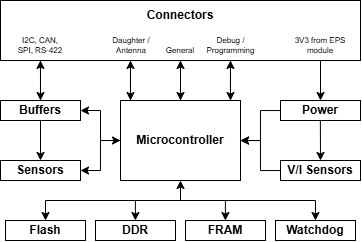
\includegraphics[scale=0.8]{images/arquitetura geral.png}
    \caption{Esquema geral de arquitetura.}
    \label{fig:arq_geral}
    \fonte{Elaboração própria.}
\end{figure}

Como podemos verificar, o microprocessador será crucial e deverá ter pinos suficientes para interface com todas as memórias, sensores e para se comunicar com os outros módulos do CubeSat. Além disso, a parte dedicada às tensões usadas deverá ser cuidadosamente feita, para suportar a potência dissipada por todos os componentes da placa de circuito impresso. A escolha de cada componente será descrita nas seções a seguir, respeitando sempre os seguintes critérios:

\begin{itemize}
	\item O componente deve funcionar corretamente nas temperaturas entre -40°C e 85°C;
	\item Circuitos integrados devem possuir herança de voo sempre que possível;
	\item Caso o circuito integrado necessite de um circuito específico, o mesmo deve conter itens preferencialmente dispostos na ECSS-Q-ST-60C, na NPSL ou similar aos mesmos, especialmente componentes discretos (capacitores, resistores, indutores, diodos, transistores, entre outros);
\end{itemize}

\subsection{Microcontrolador}

Como visto na Tabela \ref{tab:Tab_Missoes}, a fabricante com maior herança de voo estudada é a Xilinx, em especial os chips da família Zynq 7000, que são SoCs (\textit{System on a Chip}). Após um estudo próprio, o SoC Zynq 7030 se mostrou mais adequado pelas seguintes características:

\begin{itemize}
	\item Foi usado em missões extensivas em pequenos satélites (Gomspace, 2024), ou seja, possui herança de voo em missões similares em LEO e em CubeSats;
	\item Possui um envelopamento com 484 pinos, suficiente para prover as conexões necessárias para todas as interfaces requeridas (UG865, 2021);
	\item Capaz de rodar um sistema Linux (KADI et al.,2013);
	\item Por ser um SoC, possui alta adaptabilidade e flexibilidade, disponibilizando no mesmo chip uma FPGA (\textit{Field-Programmable Gate Array}) e um microprocessador, denominados respectivamente de PL e PS;
\end{itemize}

\subsection{Memórias}

As memórias serão necessárias para realizar operações, armazenar dados externos e internos e armazenar parâmetros de configuração do OBDH e de outros subsistemas do CubeSat. Para cada uma dessas funções uma memória diferente é necessária, seguindo suas características principais, sendo elas: tempo de acesso, tamanho do armazenamento e volatilidade.

\subsubsection{Memórias voláteis}

Partindo do princípio que a robustez e versatilidade estão alinhadas com a velocidade da memória, bem como sua capacidade de armazenamento máximo, a principal opção se tornou as memórias do tipo DDR (\textit{Double Data Rate}), que utilizam ambas a borda de subida e de descida para transferência de dados, atingindo o dobro de largura de banda de uma memória com SDR (\textit{Single Data Rate}) para uma mesma frequência de relógio (JEDEC, 2008). Essa relação pode ser ilustrada pela Figura \ref{fig:sdrvsddr}, onde pode-se verificar a transferência de dados do sinal DQ em relação ao sinal de relógio (bCLK e CLK) para SDR e DDR.

\begin{figure}[H]
    \centering
    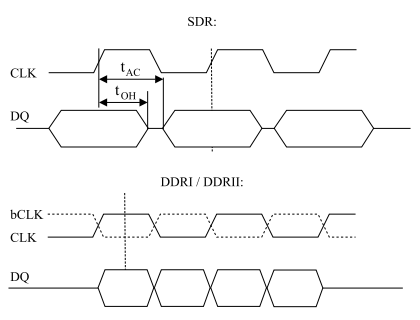
\includegraphics[scale=1]{images/ddrsdr.png}
    \caption{Comparação entre DDR e SDR.}
    \label{fig:sdrvsddr}
    \fonte{KLEHN E BROX, 2003.}
\end{figure}
 
Por essa razão, foi escolhida uma memória do tipo DDR3, com capacidade de 2Gb e frequência de operação de 800 MHz.

\subsubsection{Memórias não voláteis}

No caso das memórias não voláteis, é necessária uma atenção especial ao tipo de dado que será armazenado em cada uma delas. Para o caso de dados críticos, é preciso de uma memória que possua alta resistência aos efeitos da radiação, mantendo-se um compromisso com os tempos de escrita e leitura. Por sua vez, para dados de inicialização são mais críticos os tempos de leitura, enquanto para uma memória de dados mais gerais, o importante é o armazenamento total. Por meio desses critérios, foi possível avaliar, por meio da Tabela \ref{tab:memnvol}, o tipo de memória ideal para cada caso, considerando o número máximo de ciclos de leitura e escrita de cada tipo de memória.

\begin{table}[H]
	\ABNTEXfontereduzida
	\caption{\label{tab:memnvol}Tabela comparativa de memórias não voláteis.}
	%\begin{tabular}{@{}p{2cm}p{2cm}p{2cm}p{2cm}p{2cm}p{2cm}p{3cm}@{}}
    \centering
    \begin{tabular}{@{} >{\centering}p{2cm} >{\centering}p{3cm} >{\centering}p{3cm} >{\centering}p{3cm}>{\centering}p{3cm} @{}}
    
		\toprule
		\textbf{Memória} & \textbf{Tempo de leitura/escrita} & \textbf{Tolerância à radiação} & \textbf{Armazenamento máximo} & \textbf{Ciclos} \tabularnewline 
        \midrule
        Flash NOR & \textasciitilde{} 1$\mu$s & Ruim & \textasciitilde{} 1 Gb & \textbf{$10^5$} \tabularnewline
        
        \midrule
        Flash NAND & \textasciitilde{} 100 $\mu$s & Ruim &\textasciitilde{} 1 Tb & \textbf{$10^5$} \tabularnewline 

        \midrule
        FRAM & \textasciitilde{} 50 ns & Boa & \textasciitilde{} 1 Mb & \textbf{$10^{15}$}  \tabularnewline 
        
        \bottomrule
	\end{tabular}
	\fonte{Elaboração própria com base em (GERARDIN E PACCAGNELLA, 2010) e (BOUKHOBZA E OLIVIER, 2017).}
\end{table}

Com isso, foi então escolhida uma FRAM (\textit{Ferroelectric Random-Access Memory}) para armazenar dados críticos, uma Flash NAND para armazenamento de dados gerais e uma Flash NOR para armazenar o boot do sistema Linux no SoC.

\subsection{Conversores DC-DC}
Nos sistemas CubeSat do SpaceLab da UFSC, o módulo responsável pelo fornecimento de potência é o chamado EPS (MARCELINO, 2024). A partir disso, partindo do pressuposto que haverá uma tensão fornecida de 3,3 V, pode-se inferir a cascata de potência a partir do mesmo. Para o caso do Zynq e da memória DDR3, circuitos integrados são necessários para gerar as seguintes tensões: 

\begin{itemize}
	\item Zynq: 1 V e 1,8 V; 
	\item DDR3L: 1,35 V e 0,675 V.
\end{itemize}

Todos os demais periféricos devem aceitar uma tensão de alimentação de 3,3 V. Outro ponto importante são os circuitos de proteção contra \textit{latch-up}, um efeito similar a um curto-circuito na trilha de alimentação de circuitos CMOS (AN-600, 1989). Essa proteção é essencial, pois ao ocorrer, gera um consumo elevado de corrente e consequentemente tem potencial de gerar efeitos e falhas catastróficas (ECSS, 2018). No caso desse projeto, será utilizado o LTC4361, anteriormente usado em outras PCBs do SpaceLab, como o OBDH da  segunda geração (MARCELINO, 2024). 

Na Figura \ref{fig:diapower}, está esquematizado o sistema de potência proposto.

\begin{figure}[H]
    \centering
    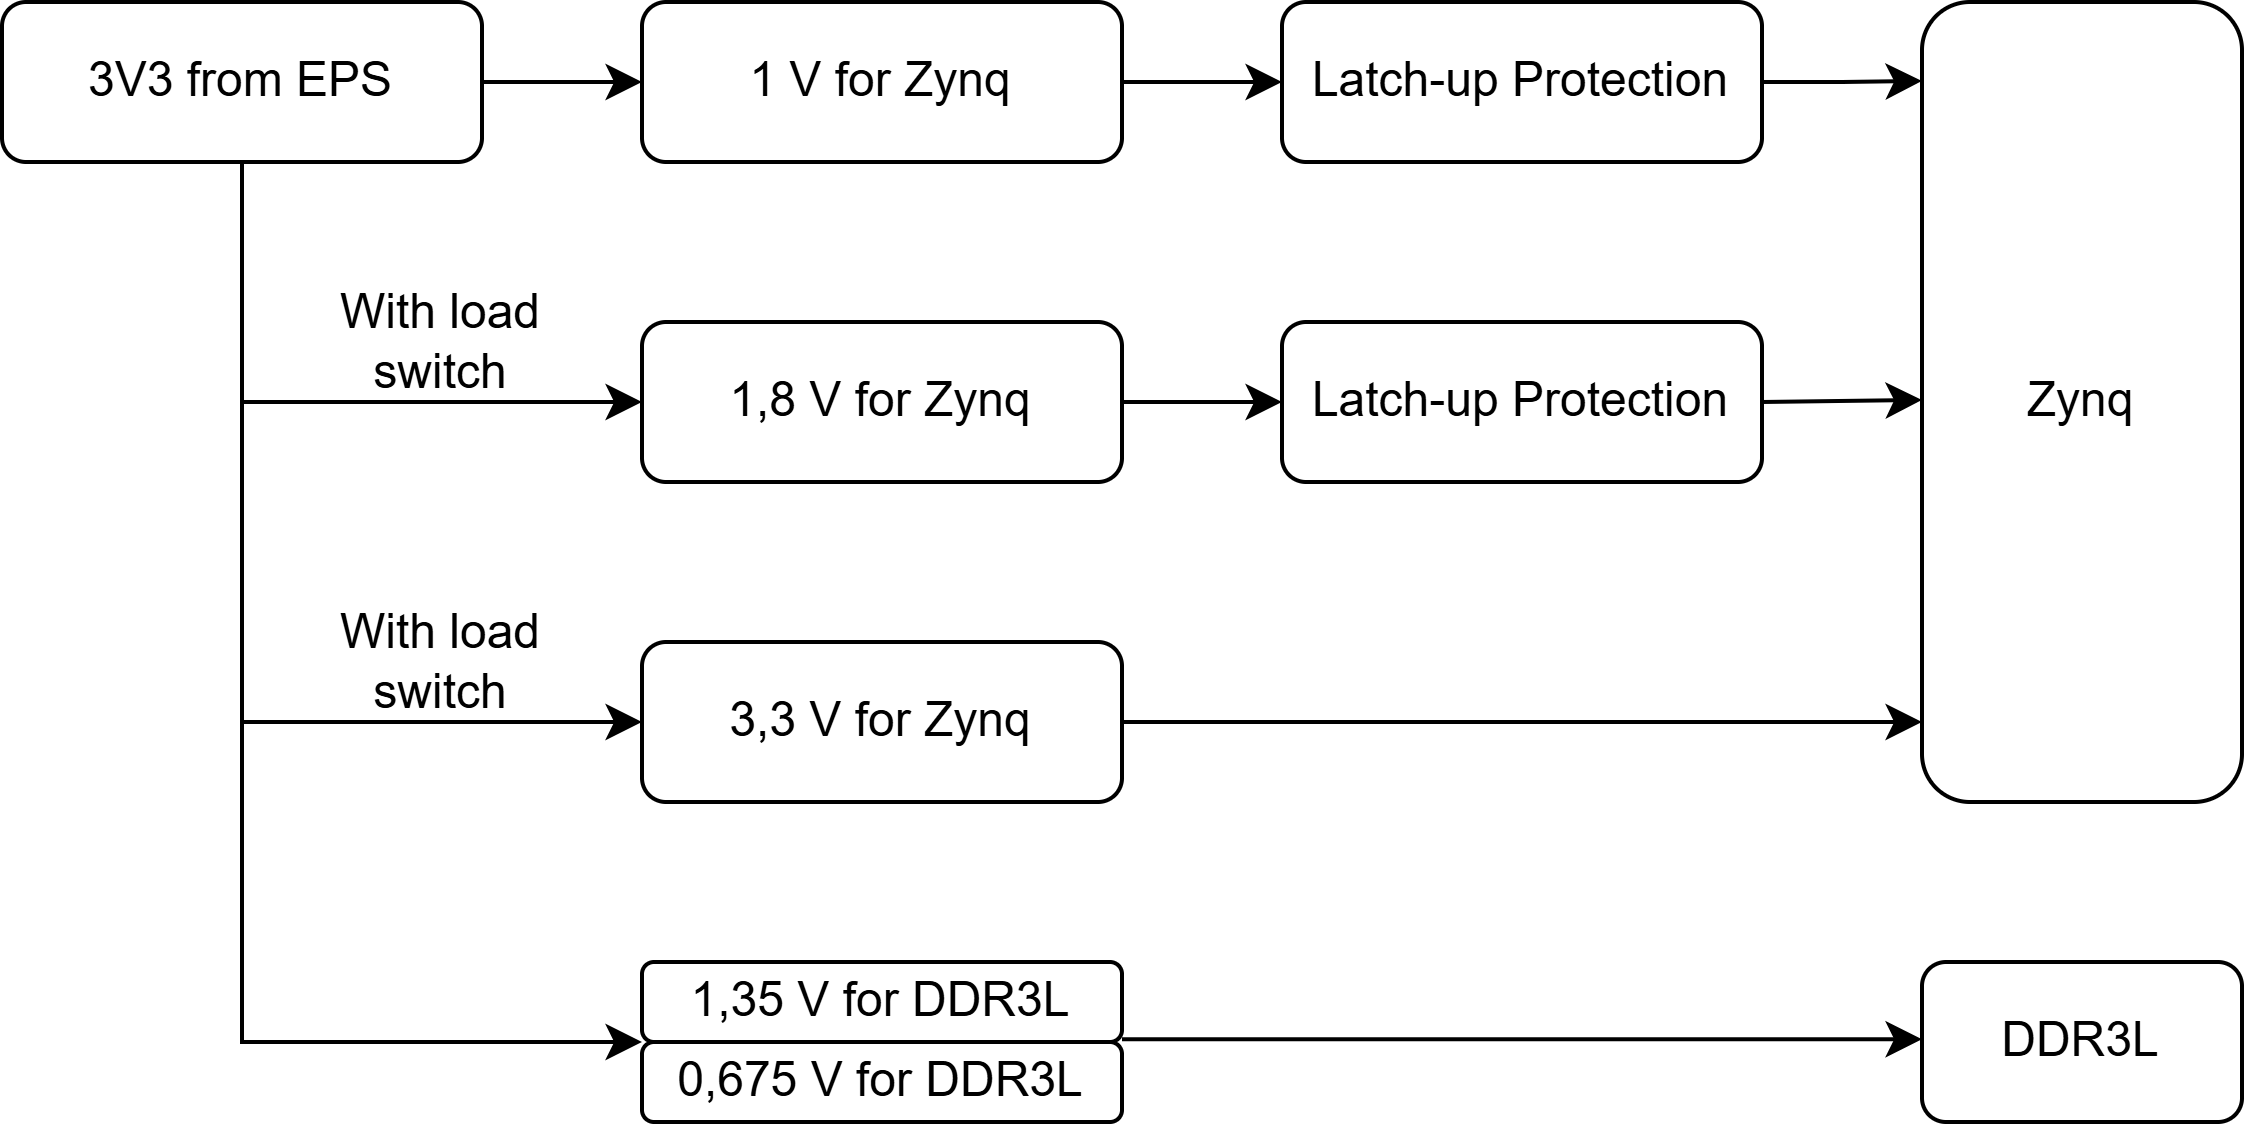
\includegraphics[scale=0.8]{images/diapower.png}
    \caption{Sistema de potência proposto.}
    \label{fig:diapower}
    \fonte{Elaboração própria.}
\end{figure}

\subsection{Sensores e Periféricos}
Como dito nos pré-requisitos, alguns sensores precisam estar presentes no OBDH. Entre eles:

\begin{itemize}
	\item Um monitor de tensão, para todas as tensões importantes do sistema;
	\item Um sensor de corrente para a tensão de entrada do módulo;
	\item Um giroscópio para medir a velocidade angular em órbita;
	\item Um magnetômetro para medição do campo magnético da Terra em órbita;
	\item Um WDT para reiniciar o sistema em caso de falha de software.
\end{itemize}

\section{Visualização da Arquitetura Proposta}

Depois das decisões tomadas, foi possível montar um diagrama, apresentado na Figura \ref{fig:arq}, que mostra cada circuito do computador de bordo. Aqui, por simplicidade, foram suprimidos os transceptores do protocolo CAN (\textit{Controller Area Network}) e a parte de potência do módulo. 

\begin{figure}[H]
    \centering
    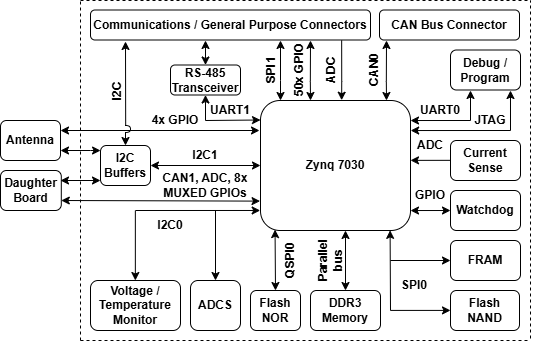
\includegraphics[scale=0.8]{images/arquitetura final.png}
    \caption{Arquitetura proposta para o OBDH.}
    \label{fig:arq}
    \fonte{Elaboração própria.}
\end{figure}

Também foram levadas em consideração as interfaces disponibilizadas pelo SoC, os componentes escolhidos e os conectores necessários. Os componentes escolhidos se encontram na Tabela \ref{tab:componentes}, conjuntamente com as interfaces requeridas para cada um, suas tensões de alimentação e suas correntes máximas no terminal de alimentação, no pior caso especificado pelo fabricante.

\begin{table}[H]
	\ABNTEXfontereduzida
	\caption{\label{tab:componentes}Informações sobre os componentes escolhidos.}
	%\begin{tabular}{@{}p{2cm}p{2cm}p{2cm}p{2cm}p{2cm}p{2cm}p{3cm}@{}}
    \centering
    \begin{tabular}{@{} >{\centering}p{2cm} >{\centering}p{4cm} >{\centering}p{2cm} >{\centering}p{3cm}>{\centering}p{3cm} @{}}
    
		\toprule
		\textbf{Componente} & \textbf{Número do Fabricante} & \textbf{Interface} & \textbf{Tensão de Alimentação} & \textbf{Corrente máxima} \tabularnewline 
        \midrule
        FRAM & CY15B104QN-50SXI & SPI & 3,3 V & 3,7 mA \tabularnewline
        
        \midrule
        Flash NOR & MT25QL128ABB1ESE-0AUT & QSPI & 3,3 V & 55 mA \tabularnewline 

        \midrule
        Flash NAND & MT29F1G01ABAFDSF-AAT:F & SPI & 3,3 V & 35 mA \tabularnewline 

        \midrule
        DDR3L & MT41K256M8DA-125:K & Paralela & 1,35 V & 182 mA \tabularnewline 

        \midrule
        WDT & TPS3823-33QDBVRQ1 & - & 3,3 V & 10 mA \tabularnewline 

        \midrule
        Monitor de Temperatura e Tensão & LTC2991IMS\#TRPBF & I2C & 3,3 V &  1,5 mA \tabularnewline 

        \midrule
        Sensor de Corrente & INA180A2IDBVR & - & 3,3 V & 1 mA \tabularnewline 

        \midrule
        Giroscópio & A3G4250D & I2C & 3,3 V & 7 mA \tabularnewline 

        \midrule
        Magnetômetro & MMC5983MA & I2C & 3,3 V & 0,45 mA \tabularnewline 

        \midrule
        Buffer I2C & TCA4311ADR & I2C & 3,3 V & 7 mA \tabularnewline 

        \midrule
        Transceptor CAN & A3G4250D & CAN & 3,3 V & 60 mA \tabularnewline 

        \midrule
        Transceptor RS-485 & THVD1451DR & Serial & 3,3 V & 3 mA \tabularnewline 

        \midrule
        Conversor DC-DC & TPS82085SILR & - & 3,3 V & - \tabularnewline 

        \midrule
        Conversor DC-DC para DDR3 & TPS51200DRCR & - & 3,3 V & 1 mA \tabularnewline 

        \midrule
        \textit{Load Switch} & TPS22920YZPR & - & 3,3 V & 0,2 mA \tabularnewline 
        
        \midrule
        Proteção contra \textit{Latch-up} & LTC4361 & - & - & - \tabularnewline 

        \bottomrule
	\end{tabular}
	\fonte{Elaboração própria com base nos Datasheets de cada componente.}
\end{table}

\subsection{Estimativa de Potência Consumida}

A fim de garantir o funcionamento correto dos conversores DC-DC e seus respectivos periféricos, foi necessária uma estimativa da potência total consumida por todas as tensões disponíveis no módulo. Para isso, foi utilizada a Tabela \ref{tab:componentes}, bem como o datasheet de cada componente. No caso do SoC, sua fabricante disponibiliza uma planilha (XPE, 2019) para estimativas de potência em cada tensão de alimentação. 

Com isso, foram obtidos os valores da Tabela \ref{tab:estpow}, considerando uma eficiência de conversão de 85\% (TPS82085, 2019), já incluindo as estimativas de potência e os piores casos descritos anteriormente.

\begin{table}[H]
	\ABNTEXfontereduzida
	\caption{\label{tab:estpow}Estimativas de potência consumida.}
	%\begin{tabular}{@{}p{2cm}p{2cm}p{2cm}p{2cm}p{2cm}p{2cm}p{3cm}@{}}
    \centering
    \begin{tabular}{@{} >{\centering}p{2cm} >{\centering}p{4cm} >{\centering}p{4cm} >{\centering}p{4cm}@{}}
    
		\toprule
		\textbf{Tensão [V]} & \textbf{Potência Dissipada na Tensão [W]} & \textbf{Potência dissipada na tensão de 3,3 V [W]} & \textbf{Corrente máxima da trilha [A]} \tabularnewline 
        \midrule
         1,00 & 2,20 & 2,59 & 2,20 \tabularnewline
        
        \midrule
        1,35 & 0,25 & 0,29 & 0,18 \tabularnewline 

        \midrule
        1,80 & 0,63 & 0,74 & 0,35 \tabularnewline

        \midrule
        3,3 & 7,5 & - & 2,27  \tabularnewline        

        \bottomrule
	\end{tabular}
	\fonte{Elaboração própria.}
\end{table}

Através dessas estimativas, pode-se confirmar que o sistema de potência proposto suporta os componentes escolhidos e suas tensões e variações, mesmo quando se considera o pior caso.
% ----------------------------------------------------------
\chapter{Desenvolvimento do Projeto}
% ----------------------------------------------------------

Depois das definições apresentadas e da escolha de componentes apresentada na seção anterior, foi possível construir um esquemático elétrico, que esquematiza a PCB do OBDH. Nesse capítulo, discutir-se-á circuitos específicos mais relevantes do projeto, usando o esquemático pronto, que se encontra no Anexo I.

\section{Conversores de Potência}

Partindo do princípio que o módulo EPS da terceira geração de módulos do SpaceLab será capaz de fornecer 3,3 V para o OBDH, foi proposta uma cascata de potência descrita na Figura \ref{fig:power}. Nela, são suprimidos os circuitos de proteção que serão descritos posteriormente.

\begin{figure}[H]
    \centering
    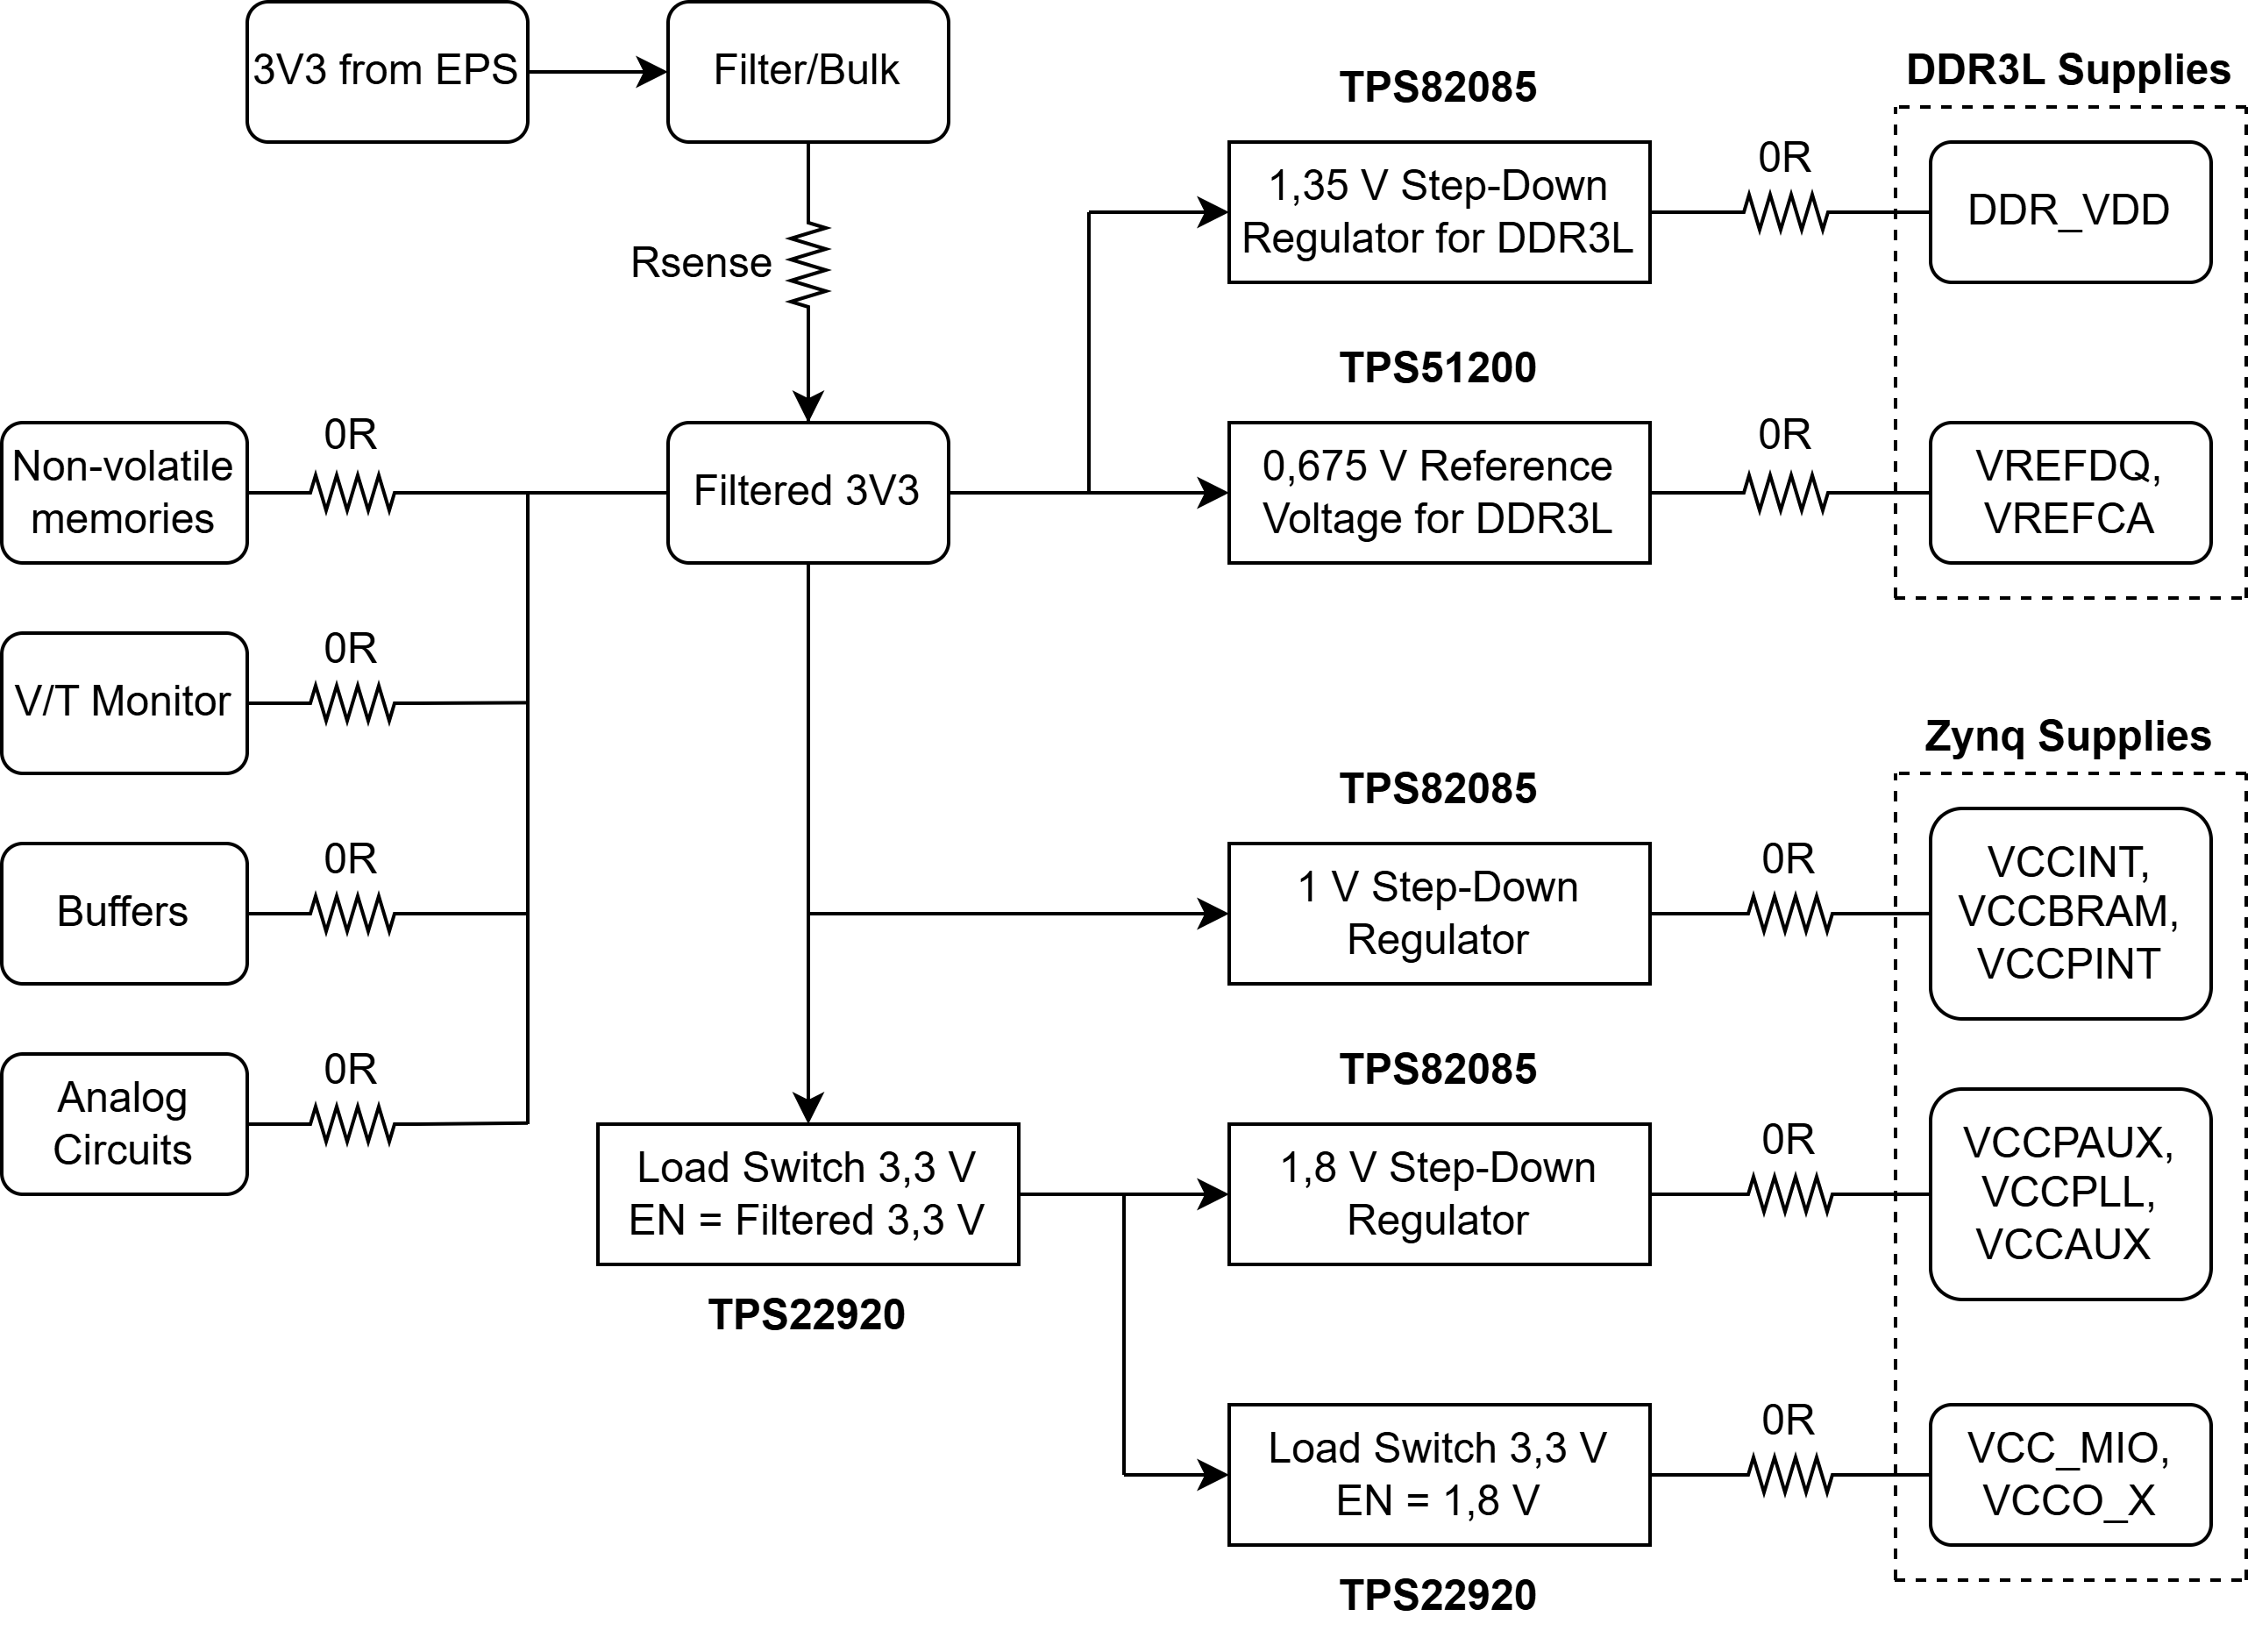
\includegraphics[scale=0.6]{images/Power_system.png}
    \caption{Cascata de potência proposta.}
    \label{fig:power}
    \fonte{Elaboração própria.}
\end{figure}

\subsection{Filtro de Entrada}

Costumeiramente, a entrada de tensão de uma placa robusta deve ser filtrada, principalmente devido às flutuações do ruído conduzido de outros subsistemas do satélite, caracterizando o fenômeno de Interferência Eletromagnética (EMI), esquematizado na Figura \ref{fig:emi}.

\begin{figure}[H]
    \centering
    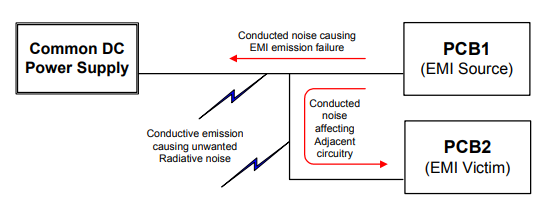
\includegraphics[scale=1]{images/EMI noise.png}
    \caption{Interferência com ruído conduzido.}
    \label{fig:emi}
    \fonte{SOH et al., 2010.}
\end{figure}

Além disso, também foi necessária a inclusão de um diodo Zener em paralelo à entrada, servindo como um elemento extra de proteção contra perturbações e transientes (CADENCE, 2023). Outra característica explorada foi a colocação de capacitores em paralelo, a fim de reduzir sua resistência em série equivalente (ESR) e sua indutância série (SARJEANT, 1990).  O filtro proposto está disposto na Figura \ref{fig:FILTRO}.  Além disso, sua magnitude e fase simuladas estão dispostas na Figura \ref{fig:filtrof}.

\begin{figure}[H]
    \centering
    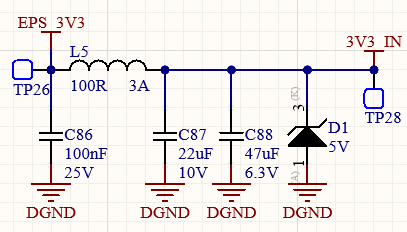
\includegraphics[scale=1]{images/FILTRO.png}
    \caption{Filtro proposto.}
    \label{fig:FILTRO}
    \fonte{Elaboração própria.}
\end{figure}

\begin{figure}[H]
    \centering
    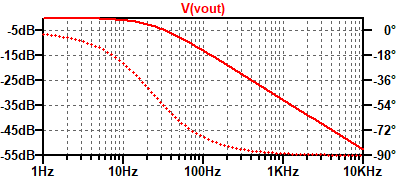
\includegraphics[scale=1]{images/filtrof.png}
    \caption{Simulação de magnitude e fase em função da frequência para o filtro proposto.}
    \label{fig:filtrof}
    \fonte{Elaboração própria.}
\end{figure}

\subsection{Cascata de potência}

Devido à escolha do SoC e da memória DDR3, foi necessária a definição de uma cascata de potência, levando-se em consideração os requisitos de (UG585, 2023), que descreve o sequenciamento das tensões para o menor consumo de potência e para garantir a integridade do fusível interno do SoC. Dessa forma, como pode-se ver na Figura \ref{fig:power}, são usados os denominados \textit{load switches}, a fim de garantir o sequenciamento descrito e garantir uma proteção efetiva contra sobrecorrente (MAK, 2018). 

O primeiro regulador, que gera a tensão de 1 V, apresentado na Figura \ref{fig:1vsupp}, é o primeiro da cascata. Seu divisor de tensão de saída foi calculado conforme (TPS82085, 2019):

\begin{equation}
	V_{out} = 0,8 * (1 + R_1/R_2) = 0,8 * (1+ 37,4k/150k) = 0,999 V
\end{equation} 

\begin{figure}[H]
    \centering
    \includegraphics[scale=0.8]{images/1vsupp.png}
    \caption{Regulador de tensão de 1 V.}
    \label{fig:1vsupp}
    \fonte{Elaboração própria com base no circuito apresentado pelo fabricante.}
\end{figure}

Também foi possível montar seu circuito de proteção de sobrecorrente, disposto na Figura \ref{fig:1vocp}. Seu resistor de entrada, que escolhe o limiar de corrente permitido, foi caculado conforme (LTC4361, 2018), considerando uma corrente 20\% superior à máxima calculada (na Tabela \ref{tab:estpow}):

\begin{equation}
	R_{sense} = 50 mV / I_{max} =50 / 2,63 = 19,01 m\Omega
\end{equation} 

\begin{figure}[H]
    \centering
    \includegraphics[scale=1]{images/1vocp.png}
    \caption{Proteção contra \textit{latch-up} para a tensão de 1 V.}
    \label{fig:1vocp}
    \fonte{Elaboração própria com base no circuito apresentado pelo fabricante.}
\end{figure}

Depois disso, para seguir com o sequenciamento requerido pelo SoC, precisa-se de um circuito de chaveamento de carga, apresentado na Figura \ref{fig:sw1}. Seu circuito é baseado no sugerido por (TPS22920, 2016), com seu ligamento sendo feito pela própria tensão de 3,3 V.

\begin{figure}[H]
    \centering
    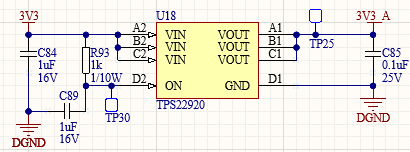
\includegraphics[scale=1]{images/sw1.png}
    \caption{Circuito de \textit{Load switch} para a tensão de 1,8 V.}
    \label{fig:sw1}
    \fonte{Elaboração própria com base no circuito apresentado pelo fabricante.}
\end{figure}

Analogamente, para a tensão de 1,8 V, são necessários ambos um conversor e um circuito de proteção. Estes estão dispostos respectivamente nas Figuras \ref{fig:1v8supp} e \ref{fig:1v8ocp} a seguir, conjuntamente com suas equações (3) e (4) para obtenção das resistências requeridas, usando a mesma margem de 20\% de corrente máxima. 

\begin{equation}
	V_{out} = 0,8 * (1 + R_1/R_2) = 0,8 * (1+ 110k/88,7k) = 1,792 V
\end{equation} 

\begin{figure}[H]
    \centering
    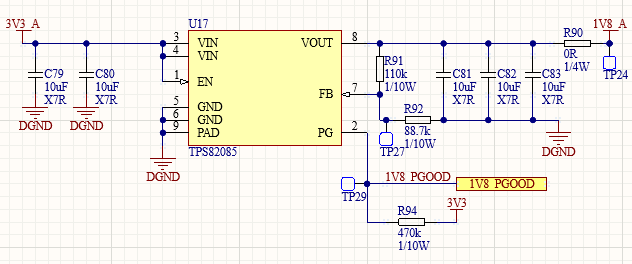
\includegraphics[scale=0.8]{images/1v8supp.png}
    \caption{Regulador de tensão de 1,8 V.}
    \label{fig:1v8supp}
    \fonte{Elaboração própria com base no circuito apresentado pelo fabricante.}
\end{figure}

\begin{equation}
	R_{sense} = 50 mV / I_{max} =50 / 0,5 = 100 m\Omega
\end{equation} 

\begin{figure}[H]
    \centering
    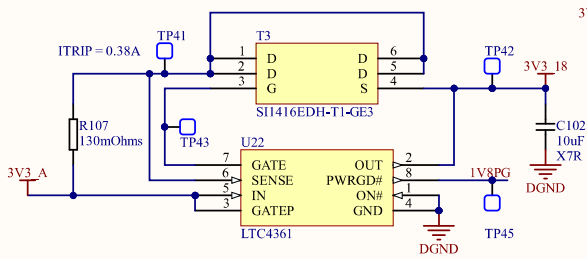
\includegraphics[scale=1]{images/1v8ocp.png}
    \caption{Proteção contra \textit{latch-up} para a tensão de 1,8 V.}
    \label{fig:1v8ocp}
    \fonte{Elaboração própria com base no circuito apresentado pelo fabricante.}
\end{figure}

Por fim, para ligar a tensão de 3,3 V fornecida para o SoC, é necessário um último circuito de chaveamento, dessa vez com seu ligamento feito pela tensão de 1,8 V, como mostra a Figura \ref{fig:sw2}.

\begin{figure}[H]
    \centering
    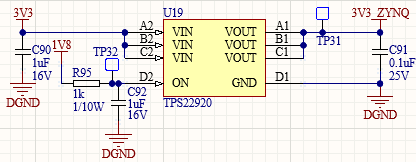
\includegraphics[scale=1]{images/sw2.png}
    \caption{Circuito de \textit{Load switch} para a tensão de 3,3 V do SoC.}
    \label{fig:sw2}
    \fonte{Elaboração própria com base no circuito apresentado pelo fabricante.}
\end{figure}

Paralelamente, para a memória DDR3L, são necessários um conversor para a alimentação, de 1,35 V, e um conversor para a tensão de referência e de terminação. Esses circuitos estão dispostos respectivamente nas Figuras \ref{fig:1v35supp} e \ref{fig:1v35ref}.

\begin{equation}
	V_{out} = 0,8 * (1 + R_1/R_2) = 0,8 * (1+ 47k/68k) = 1,353 V
\end{equation} 

\begin{figure}[H]
    \centering
    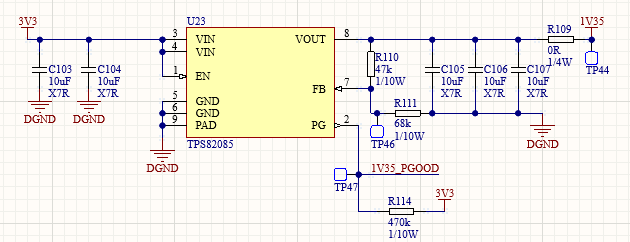
\includegraphics[scale=0.8]{images/1v35supp.png}
    \caption{Regulador de tensão de 1,35 V.}
    \label{fig:1v35supp}
    \fonte{Elaboração própria com base no circuito apresentado pelo fabricante.}
\end{figure}

\begin{figure}[H]
    \centering
    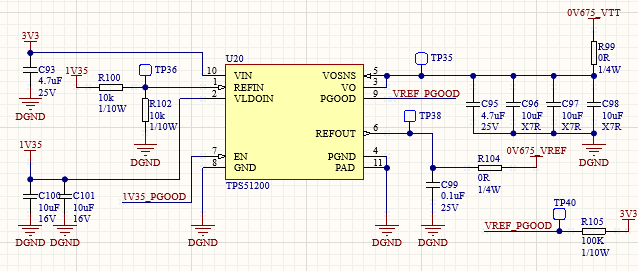
\includegraphics[scale=0.8]{images/refsupp.png}
    \caption{Regulador de tensão de referência e terminação para a memória DDR3L.}
    \label{fig:1v35ref}
    \fonte{Elaboração própria com base no circuito apresentado pelo fabricante.}
\end{figure}

\section{SoC}

No caso do SoC Zynq 7030, temos no total seis blocos operacionais, que incluem o funcionamento do PL e do PS, bem como as configurações e o bloco dedicado ao controlador da memória DDR (UG585, 2023). A seguir, estão dispostas as descrições funcionais e circuitos necessários para o funcionamento correto desse SoC, separados por cada um dos blocos citados.

\subsection{Bloco de Configuração}

O banco zero do SoC é o responsável por algumas opções e sinais de configuração. Abaixo, na Tabela \ref{tab:config}, se encontra a descrição funcional de cada pino desse banco, esquematizado na Figura \ref{fig:config}. Esse esquemático, bem como seus resistores de \textit{pull-up} (Figura \ref{fig:pullupconfig}), foram baseados na documentação técnica fornecida pela Xilinx (UG865, 2023) (UG470, 2023) (UG933, 2019) (DS191, 2018).


\begin{table}[H]
	\ABNTEXfontereduzida
	\caption{\label{tab:config}Descrição funcional dos pinos de configuração.}
	%\begin{tabular}{@{}p{2cm}p{2cm}p{2cm}p{2cm}p{2cm}p{2cm}p{3cm}@{}}
    \centering
    \begin{tabular}{@{} >{\centering}p{4cm} >{\centering}p{8cm} @{}}
    
		\toprule
		\textbf{Nome} & \textbf{Função} \tabularnewline 
        \midrule
         DXN e DXP & Terminais do diodo interno para medição de temperatura. \tabularnewline
         \midrule

         VREFP e VREFN & Tensões de referência do conversor analógico digital (XADC) do SoC. \tabularnewline

       \midrule
        VP e VN & Entrada extra do XADC. \tabularnewline

       \midrule
        VCCBAT & Não utilizada. Fonte da bateria. \tabularnewline

       \midrule
        TCK, TMS, TDI e TDO & Sinais da interface JTAG.  \tabularnewline

       \midrule
        INIT\_B & Indica inicialização da memória interna de configuração. \tabularnewline

       \midrule
       PROGRAM\_B & Reset assíncrono da lógica de configuração. \tabularnewline

       \midrule
        CFGBVS & Pino que seleciona o tipo de IO do banco 0. \tabularnewline

       \midrule
        DONE & Indica que a configuração foi terminada e feita corretamente. \tabularnewline

       \midrule
        VCCADC e GNDADC & Alimentação do XADC. \tabularnewline

       \midrule
        RSVDVCC e RSVDGND & Pinos de alimentação reservados. \tabularnewline

        \bottomrule
	\end{tabular}
	\fonte{Elaboração própria com base na documentação técnica do fabricante.}
\end{table}

\begin{figure}[H]
    \centering
    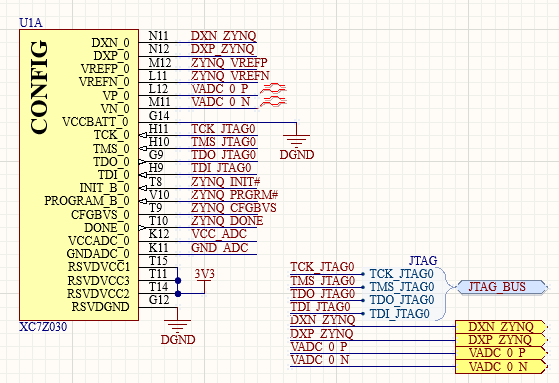
\includegraphics[scale=0.8]{images/zynqconfig.png}
    \caption{Banco de configuração do SoC.}
    \label{fig:config}
    \fonte{Elaboração própria com base no circuito apresentado pelo fabricante.}
\end{figure}

\begin{figure}[H]
    \centering
    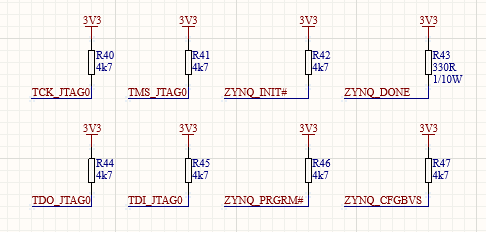
\includegraphics[scale=0.8]{images/pullupconfig.png}
    \caption{Resistores de \textit{pull-up} necessários.}
    \label{fig:pullupconfig}
    \fonte{Elaboração própria com base no circuito apresentado pelo fabricante.}
\end{figure}

Além disso, para a alimentação do XADC, foi necessário um circuito de filtragem, disposto na Figura \ref{fig:xadcfilter}, como requerido por (UG480, 2022).

\begin{figure}[H]
    \centering
    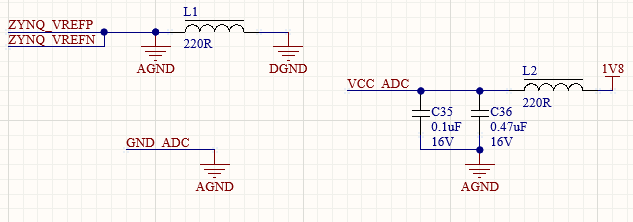
\includegraphics[scale=0.8]{images/xadcfilter.png}
    \caption{Filtro da alimentação analógica do SoC.}
    \label{fig:xadcfilter}
    \fonte{Elaboração própria com base no circuito apresentado pelo fabricante.}
\end{figure}


\subsection{Blocos do PS}

No caso do sistema de processamento (PS), temos dois bancos principais. O primeiro, denominado MIO (\textit{Multiplexed In-Out}), é onde se encontram os controladores das interfaces de comunicação, bem como a entrada de relógio e a escolha do \textit{boot}. No caso desse projeto, foi-se decidido que o SoC poderá inicializar de duas formas, sendo a primeira pela interface JTAG e a segunda pela memória Flash NOR (QSPI), escolhidos pelos resistores R48 e R51. O banco MIO e seus modos de inicialização estão dispostos nas Figuras \ref{fig:psmio} e \ref{fig:boot}. O outro banco do PS (112) não é utilizado nesse projeto.

\begin{figure}[H]
    \centering
    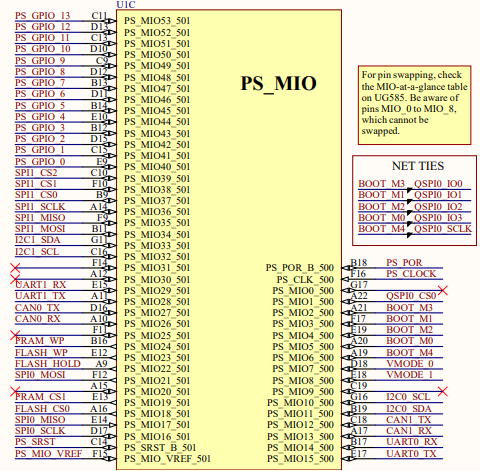
\includegraphics[scale=0.8]{images/psmio.png}
    \caption{Banco MIO do SoC com suas respectivas entradas e saídas.}
    \label{fig:psmio}
    \fonte{Elaboração própria com base na Tabela MIO-at-a-glance (UG585, 2023).}
\end{figure}

\begin{figure}[H]
    \centering
    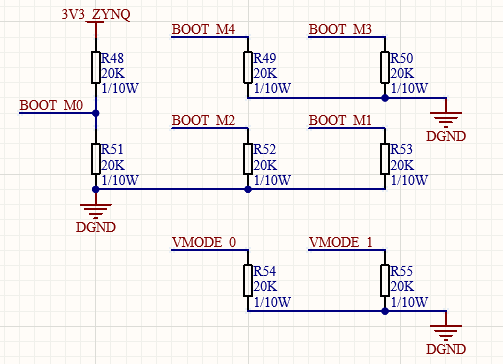
\includegraphics[scale=0.8]{images/bootmode.png}
    \caption{Modos de inicialização do SoC.}
    \label{fig:boot}
    \fonte{Elaboração própria com base em (UG585, 2023).}
\end{figure}

Por fim, Na Tabela \ref{tab:interfaces}, pode-se verificar qual a função de cada barramento de comunicação, em conformidade com a Figura \ref{fig:arq}. 

\begin{table}[H]
	\ABNTEXfontereduzida
	\caption{\label{tab:interfaces}Descrição das interfaces disponibilizadas.}
	%\begin{tabular}{@{}p{2cm}p{2cm}p{2cm}p{2cm}p{2cm}p{2cm}p{3cm}@{}}
    \centering
    \begin{tabular}{@{} >{\centering}p{4cm} >{\centering}p{8cm} @{}}
    
		\toprule
		\textbf{Interface} & \textbf{Função} \tabularnewline 
        \midrule
         SPI0 & Interface SPI para circuitos internos ao módulo OBDH. \tabularnewline
        \midrule
         SPI1 & Interface SPI para circuitos externos ao módulo OBDH.  \tabularnewline
        \midrule
         QSPI0 & Interface Quad-SPI para memória de inicialização. \tabularnewline
        \midrule
        I2C0  & Interface I2C para circuitos internos ao módulo OBDH. \tabularnewline
        \midrule
        I2C1  & Interface I2C para circuitos externos ao módulo OBDH.  \tabularnewline
        \midrule
        CAN0 & Interface CAN para circuitos externos ao módulo OBDH. \tabularnewline
        \midrule
        CAN1 & Interface CAN para o módulo \textit{daughter}. \tabularnewline
        \midrule
         UART0 & Conexão serial para \textit{debugging}. \tabularnewline
        \midrule
         UART1 & Conexão serial para o transceiver RS-485. \tabularnewline
        \midrule
         PS\_GPIO & Sinais de propósito geral de entrada e saída. \tabularnewline

        \bottomrule
	\end{tabular}
	\fonte{Elaboração própria com base na documentação técnica do fabricante.}
\end{table}

\subsection{Blocos do PL}

\subsection{Bloco Controlador da Memória DDR}

\subsection{Pinos de Potência}

\section{Conexões entre blocos}
\begin{flushleft}
\begin{thebibliography}{00} %59
\bibitem{b1} AAC Clyde Space. \textbf{Datasheet: Kryten-M3}. Disponível em $<$https://www.aac-clyde.space/wp-content/uploads/2021/10/AAC\_DataSheet\_Kryten.pdf$>$.  Acesso em: 07 jun. 2024.

\bibitem{b36} \textbf{A3G4250D Gyroscope Datasheet}. Disponível em: $<$\url{https://www.st.com/content/ccc/resource/technical/document/datasheet/5c/f1/a4/70/1b/fa/40/d2/DM00047823.pdf/files/DM00047823.pdf/jcr:content/translations/en.DM00047823.pdf}$>$. Acesso em: 27 out. 2024. 

\bibitem{b21} \textbf{AN-600: Understanding Latch-Up in Advanced CMOS Logic}. [s.l: s.n.]. Disponível em: $<$https://large.stanford.edu/courses/2015/ph241/clark2/docs/AN-600.pdf$>$. Acesso em: 26 out. 2024.

\bibitem{b48} BARLES, A. et al. \textbf{Mission ORCA: Orbit refinement for collision avoidance}. Advances in Astronautics Science and Technology, v. 5, n. 2, p. 149–165, 2022.

%\bibitem{b57} BOING, M. \textbf{Técnicas de mitigação de efeitos da radiação e sua aplicação no projeto de uma arquitetura de hardware para uso em satélites}. Florianópolis, SC: UFSC, 19 de julho de 2024.

\bibitem{b56} BOUKHOBZA, J.; OLIVIER, P. \textbf{Emerging Non-volatile Memories}. Em: Flash Memory Integration. [s.l.] Elsevier, 2017. p. 203–224.

\bibitem{b40} CADENCE PCB SOLUTIONS. \textbf{Zener diode applications: Circuit protection}. Disponível em: <https://resources.pcb.cadence.com/blog/2023-zener-diode-applications-circuit-protection>. Acesso em: 28 out. 2024

\bibitem{b13} CARMO, T. A.; MOREIRA , J. Q.; MANEA, S. \textbf{Análise de blindagem à radiação “TID” e “SEU” em memória do tipo SRAM em orbita LEO (Low Earth Orbit)}. 12° Workshop em Engenharia e Tecnologia Espaciais, 6 nov. 2021.

\bibitem{b49} CAMPS, A. et al. \textbf{Fsscat, the 2017 Copernicus masters’ “Esa sentinel small satellite challenge” winner: A federated polar and soil moisture tandem mission based on 6U cubesats}. IGARSS 2018 - 2018 IEEE International Geoscience and Remote Sensing Symposium. Anais...IEEE, 2018.

\bibitem{b2} CAPPELLETTI, C.; BATTISTINI, S.; MALPHRUS, B. \textbf{Cubesat Handbook: From Mission Design to Operations}. Editora Elsevier, 2021.

\bibitem{b58} \textit{CubeSat101: Basic Concepts and Processes for First-Time CubeSat Developers}. [S.l.: s.n.], 2017. Disponível em $<$https://www.nasa.gov/wp-content/uploads/2017/03/nasa\_csli\_cubesat\_101\_508.pdf?emrc=05d3e2$>$. Acesso em 28 out. 2024.

\bibitem{b15} \textbf{CUBESAT Design Specification}. [S.l.: s.n.], 2022. Disponível em $<$https://www.cubesat.org/cubesatinfo$>$. Acesso em: 25 out. 2024.

\bibitem{b22} \textbf{CY15B104QN FRAM Datasheet}. Disponível em: $<$\url{https://www.infineon.com/dgdl/Infineon-CY15B104QN\_CY15V104QN\_Excelon(TM)\_LP\_4-Mbit\_(512K\_X\_8)\_Serial\_(SPI)\_F-RAM-DataSheet-v12\_00-EN.pdf?fileId=8ac78c8c7d0d8da4017d0ee7709b704a\&utm\_source=cypress\&utm\_medium=referral\&utm\_campaign=202110\_globe\_en\_all\_integr}$>$. Acesso em: 27 out. 2024.

\bibitem{b47} \textbf{DS191 - Zynq-7000 SoC (Z-7030, Z-7035, Z-7045, and Z-7100): DC and AC Switching Characteristics}. 2018. Disponível em $<$https://docs.amd.com/v/u/en-US/ds191-XC7Z030-XC7Z045-data-sheet$>$. Acesso em: 29 out. 2024.

\bibitem{b14} ECSS. \textbf{ECSS-Q-ST-60C Rev.3 – Electrical, electronic and electromechanical (EEE) components (12 May 2022)}. Disponível em: $<$https://ecss.nl/standard/ecss-q-st-60c-rev-3-electrical-electronic-and-electromechanical-eee-components-2-may-2022/$>$. Acesso em: 6 out. 2024.

\bibitem{b57} ECSS. \textbf{ECSS-E-ST-10-04C - Space Environment}. The Netherlands: [s.n.], 2008.

\bibitem{b20} GERARDIN, S.; PACCAGNELLA, A. \textbf{Present and future non-volatile memories for space}. IEEE transactions on nuclear science, 2010.

\bibitem{b3} GEORGE, A. D.; WILSON, C. M. \textbf{Onboard processing with hybrid and reconfigurable computing on small satellites}. Proceedings of the IEEE. Institute of Electrical and Electronics Engineers, 2018.

\bibitem{b4} \textbf{Gomspace NanoMind A3200 Datasheet}. Disponível em $<$https://gomspace.com/UserFiles/Subsystems/datasheet/gs-ds-nanomind-a3200\_1006901-117.pdf$>$. Acesso em: 07 jun. 2024.

\bibitem{b5} \textbf{Gomspace NanoMind HP MK3 Datasheet}. Disponível em $<$https://gomspace.com/UserFiles/Subsystems/datasheet/gs-ds-NanoMind\_HP\_MK3.pdf$>$. Acesso em: 07 jun. 2024.

\bibitem{b51} \textbf{Gomspace Nanomind Z7000 Datasheet}. 2019. Disponível em: $<$https://gomspace.com/UserFiles/Subsystems/datasheet/gs-ds-nanomind-z7000-15.pdf$>$. Acesso em: 30 oct. 2024.

\bibitem{b34} \textbf{INA180A2IDBVR Current Sense Datasheet}. Disponível em: $<$\url{https://www.ti.com/lit/ds/symlink/ina180.pdf?HQS=dis-dk-null-digikeymode-dsf-pf-null-wwe\&ts=1727202734954\&ref\_url=https\%253A\%252F\%252Fwww.ti.com\%252Fgeneral\%252Fdocs\%252Fsuppproductinfo.tsp\%253FdistId\%253D10\%2526gotoUrl\%253Dhttps\%253A\%252F\%252Fwww.ti.com\%252Flit\%252Fgpn\%252Fina180}$>$. Acesso em: 27 out. 2024. 

\bibitem{b6} \textbf{ISIS Space On Board Computer}. Disponível em $<$https://www.isispace.nl/product/on-board-computer/$>$. Acesso em: 07 jun. 2024.

\bibitem{b19} JEDEC. \textbf{Double Data Rate (DDR) SDRAM Standard}. 2008. Disponível em: $<$https://www.jedec.org/standards-documents/docs/jesd-79f$>$. Acesso em: 26 out. 2024.

\bibitem{b10} JUNQUEIRA, B. C.; MANEA, S.\textbf{Utilização de COTS em nano satélites}. Brazilian Journal of Development, v. 6, n. 1, p. 1476-1490, 2020.

\bibitem{b16} KADI, M. A. et al. \textbf{Dynamic and partial reconfiguration of Zynq 7000 under Linux}. 2013 International Conference on Reconfigurable Computing and FPGAs (ReConFig). Anais...IEEE, 2013.

\bibitem{b18} KLEHN, B.; BROX, M. A. \textbf{Comparison of current SDRAM types: SDR, DDR, and RDRAM}. Advances in radio science, v. 1, p. 265–271, 2003.

\bibitem{b59} LABEL, K. A. \textbf{Radiation Effects on Electronics 101: Simple Concepts and New Challenges}. NEPP Webex Presentation, 2004.

\bibitem{b54} LOFFLER, T. et al. \textbf{Research and Observation in Medium Earth Orbit (ROMEO) with a cost-effective microsatellite platform}. 72nd International Astronautical Congress (IAC), Dubai, United Arab Emirates. 2021. 

\bibitem{b12} \textbf{Low earth orbit}. Disponível em: $<$https://www.esa.int/ESA\_Multimedia/Images/2020/03/Low\_Earth\_orbit$>$. Acesso em: 6 out. 2024.

\bibitem{b27} \textbf{LTC2991IMS\#TRPBF Voltage, Current and Temperature Monitor Datasheet}. Disponível em: $<$https://www.analog.com/media/en/technical-documentation/data-sheets/2991ff.pdf$>$. Acesso em: 27 out. 2024. 

\bibitem{b37} \textbf{LTC4361 Overcurrent Protection Controller Datasheet}. 2018. Disponível em: $<$https://www.analog.com/media/en/technical-documentation/data-sheets/LTC4361-1-4361-2.pdf$>$. Acesso em: 27 out. 2024. 

\bibitem{b11} MAYANBARI, Masood; KASESAZ, Yaser. \textbf{Design and analyse space radiation shielding for a nanosatellite in Low Earth Orbit (LEO)}. In: Proceedings of 5th International Conference on Recent Advances in Space Technologies-RAST2011. IEEE, 2011. p. 489-493.

\bibitem{b42} MAK, B. \textbf{Basics of Load Switches}. 2018. Disponível em: <https://www.ti.com/lit/an/slva652a/slva652a.pdf?ts=1730079105016>. Acesso em: 28 out. 2024.

\bibitem{b8} MARCELINO, G. M. et al. \textbf{A critical embedded system challenge: The FloripaSat-1 mission}. IEEE Latin America Transactions, 2020.

\bibitem{b9} MARCELINO, G. M. et al. \textbf{FloripaSat-2: An Open-Source Platform for CubeSats}. IEEE embedded systems letters, 2024.

\bibitem{b35} \textbf{MMC5983MA Magnetometer Datasheet}. Disponível em: $<$\url{https://mm.digikey.com/Volume0/opasdata/d220001/medias/docus/333/MMC5983MA\_RevA\_4-3-19.pdf}$>$. Acesso em: 27 out. 2024. 

\bibitem{b25} \textbf{MT25QL128ABB1ESE-0AUT Flash NOR Datasheet}. Disponível em: $<$https://www.micron.com/content/dam/micron/global/secure/products/data-sheet/nor-flash/serial-nor/mt25q/die-rev-b/mt25q-qlht-l-128-abb-xxt.pdf$>$. Acesso em: 27 out. 2024. 

\bibitem{b24} \textbf{MT29F1G01ABAFDSF-AAT:F Flash NAND Datasheet}. Disponível em: $<$https://www.micron.com/content/dam/micron/global/secure/products/data-sheet/nand-flash/70-series/m78a-1gb-spi-auto.pdf$>$. Acesso em: 27 out. 2024. 

\bibitem{b23} \textbf{MT41K256M8DA-125:K DDR3L Datasheet}. Disponível em: $<$https://www.micron.com/content/dam/micron/global/secure/products/data-sheet/dram/ddr3/2gb-1-35v-ddr3l.pdf$>$. Acesso em: 27 out. 2024. 

\bibitem{b7} Nano Avionics. \textbf{CubeSat On-Board Computer – Main Bus Unit SatBus 3C2}. Disponível em $<$https://nanoavionics.com/cubesat-components/cubesat-on-board-computer-main-bus-unit-satbus-3c2/$>$. Acesso em: 07 jun. 2024.

\bibitem{b13} \textbf{NASA Parts Selection List (NPSL)}. Disponível em: $<$https://nepp.nasa.gov/npsl/$>$. Acesso em: 6 out. 2024.

\bibitem{b55} \textbf{NASA Product Verification}. Disponível em: $<$https://www.nasa.gov/reference/5-3-product-verification/$>$. Acesso em: 30 out. 2024.

\bibitem{b53} PUTRA, A. C. A. Y.; WIJANTO, H.; EDWAR. \textbf{Design and implementation RTOS (real time operating system) as a nano satellite control for responding to space environmental conditions}. 2021 IEEE Asia Pacific Conference on Wireless and Mobile (APWiMob). Anais...IEEE, 2021.

\bibitem{b41} SARJEANT, W. \textbf{Capacitors}. IEEE transactions on electrical insulation, v. 25, n. 5, p. 861–922, 1990.

\bibitem{b39} SOH, W.-S. et al. \textbf{Filter design for suppression of noise coupling from PCB to DC power supply}. 2010 Asia-Pacific International Symposium on Electromagnetic Compatibility. Anais...IEEE, 2010.

\bibitem{b28} \textbf{TCA4311ADR I2C Buffer Datasheet}. Disponível em: $<$\url{https://www.ti.com/general/docs/suppproductinfo.tsp?distId=10\&gotoUrl=https\%3A\%2F\%2Fwww.ti.com\%2Flit\%2Fgpn\%2Ftca4311a}$>$. Acesso em: 27 out. 2024. 

\bibitem{b33} \textbf{TCAN330D CAN Transceiver Datasheet}. Disponível em: $<$\url{https://www.ti.com/lit/ds/symlink/tcan330.pdf?ts=1729084231140\&ref\_url=https\%253A\%252F\%252Fbr.mouser.com\%252F}$>$. Acesso em: 27 out. 2024. 

\bibitem{b29} \textbf{THVD1451DR RS-485 Transceiver Datasheet}. Disponível em: $<$\url{https://www.ti.com/lit/ds/symlink/thvd1410.pdf?HQS=dis-dk-null-digikeymode-dsf-pf-null-wwe\&ts=1722094226249\&ref\_url=https\%253A\%252F\%252Fwww.ti.com\%252Fgeneral\%252Fdocs\%252Fsuppproductinfo.tsp\%253FdistId\%253D10\%2526gotoUrl\%253Dhttps\%253A\%252F\%252Fwww.ti.com\%252Flit\%252Fgpn\%252Fthvd1410}$>$. Acesso em: 27 out. 2024. 

\bibitem{b30} \textbf{TPS22920YZPR Load Switch Datasheet}. 2016. Disponível em: $<$\url{https://www.ti.com/general/docs/suppproductinfo.tsp?distId=10\&gotoUrl=https\%3A\%2F\%2Fwww.ti.com\%2Flit\%2Fgpn\%2Ftps22920}$>$. Acesso em: 27 out. 2024. 

\bibitem{b26} \textbf{TPS3823-33QDBVRQ1 Watchdog Timer Datasheet}. Disponível em: $<$\url{https://www.ti.com/general/docs/suppproductinfo.tsp?distId=10\&gotoUrl=https\%3A\%2F\%2Fwww.ti.com\%2Flit\%2Fgpn\%2Ftps3828-q1}$>$. Acesso em: 27 out. 2024. 

\bibitem{b31} \textbf{TPS51200DRCR DC-DC Voltage Regulator Datasheet}. Disponível em: $<$\url{https://www.ti.com/general/docs/suppproductinfo.tsp?distId=10\&gotoUrl=https\%3A\%2F\%2Fwww.ti.com\%2Flit\%2Fgpn\%2Ftps51200}$>$. Acesso em: 27 out. 2024. 

\bibitem{b32} \textbf{TPS82085SILR DC-DC Voltage Regulator Datasheet}. 2019. Disponível em: $<$\url{https://www.ti.com/general/docs/suppproductinfo.tsp?distId=10\&gotoUrl=https\%3A\%2F\%2Fwww.ti.com\%2Flit\%2Fgpn\%2Ftps82085}$>$. Acesso em: 27 out. 2024. 

\bibitem{b44} \textbf{UG470 - 7 Series FPGAs Configuration User Guide}. 2023. Disponível em $<$https://docs.amd.com/v/u/en-US/ug470\_7Series\_Config$>$. Acesso em: 29 out. 2024.

\bibitem{b45} \textbf{UG480 - 7 Series FPGAs and Zynq-7000 SoC XADC Dual 12-Bit 1 MSPS Analog-to-Digital Converter User Guide}. 2022. Disponível em $<$https://docs.amd.com/r/en-US/ug480\_7Series\_XADC$>$. Acesso em: 29 out. 2024.

\bibitem{b38} \textbf{UG585 - Zynq 7000 SoC Technical Reference Manual - AMD technical information portal}. 2023. Disponível em: $<$https://docs.amd.com/r/en-US/ug585-zynq-7000-SoC-TRM/Zynq-7000-SoC-Technical-Reference-Manual$>$. Acesso em: 25 out. 2024.

\bibitem{b17} \textbf{UG865 - Zynq-7000 SoC Packaging and Pinout Product Specification - AMD technical information portal}. 2021. Disponível em: $<$https://docs.amd.com/v/u/en-US/ug865-Zynq-7000-Pkg-Pinout$>$. Acesso em: 25 out. 2024.

\bibitem{b46} \textbf{UG933 - Zynq-7000 SoC PCB Design Guide}. 2019. Disponível em $<$https://docs.amd.com/v/u/en-US/ug933-Zynq-7000-PCB$>$. Acesso em: 29 out. 2024.

\bibitem{b50} WEIDMANN, D. et al. \textbf{Cubesats for monitoring atmospheric processes (CubeMAP): a constellation mission to study the middle atmosphere}. Sensors, Systems, and Next-Generation Satellites XXIV. Anais...SPIE, 2020.

\bibitem{b43} \textbf{XPE - Power Estimator}. 2019. Disponível em: $<$https://www.amd.com/en/products/adaptive-socs-and-fpgas/technologies/power-efficiency/power-estimator.html$>$. Acesso em: 28 out. 2024.

\bibitem{b52} ZHOU, Q. et al. \textbf{Design of a compact and reconfigurable onboard data handling system}. 2018 IEEE Intl Conf on Parallel \& Distributed Processing with Applications, Ubiquitous Computing \& Communications, Big Data \& Cloud Computing, Social Computing \& Networking, Sustainable Computing \& Communications (ISPA/IUCC/BDCloud/SocialCom/SustainCom). Anais...IEEE, 2018.

\end{thebibliography}
\end{flushleft}


\postextual
%\begin{flushleft}
\begin{thebibliography}{00} %59
\bibitem{b1} AAC Clyde Space. \textbf{Datasheet: Kryten-M3}. Disponível em $<$https://www.aac-clyde.space/wp-content/uploads/2021/10/AAC\_DataSheet\_Kryten.pdf$>$.  Acesso em: 07 jun. 2024.

\bibitem{b36} \textbf{A3G4250D Gyroscope Datasheet}. Disponível em: $<$\url{https://www.st.com/content/ccc/resource/technical/document/datasheet/5c/f1/a4/70/1b/fa/40/d2/DM00047823.pdf/files/DM00047823.pdf/jcr:content/translations/en.DM00047823.pdf}$>$. Acesso em: 27 out. 2024. 

\bibitem{b21} \textbf{AN-600: Understanding Latch-Up in Advanced CMOS Logic}. [s.l: s.n.]. Disponível em: $<$https://large.stanford.edu/courses/2015/ph241/clark2/docs/AN-600.pdf$>$. Acesso em: 26 out. 2024.

\bibitem{b48} BARLES, A. et al. \textbf{Mission ORCA: Orbit refinement for collision avoidance}. Advances in Astronautics Science and Technology, v. 5, n. 2, p. 149–165, 2022.

%\bibitem{b57} BOING, M. \textbf{Técnicas de mitigação de efeitos da radiação e sua aplicação no projeto de uma arquitetura de hardware para uso em satélites}. Florianópolis, SC: UFSC, 19 de julho de 2024.

\bibitem{b56} BOUKHOBZA, J.; OLIVIER, P. \textbf{Emerging Non-volatile Memories}. Em: Flash Memory Integration. [s.l.] Elsevier, 2017. p. 203–224.

\bibitem{b40} CADENCE PCB SOLUTIONS. \textbf{Zener diode applications: Circuit protection}. Disponível em: <https://resources.pcb.cadence.com/blog/2023-zener-diode-applications-circuit-protection>. Acesso em: 28 out. 2024

\bibitem{b13} CARMO, T. A.; MOREIRA , J. Q.; MANEA, S. \textbf{Análise de blindagem à radiação “TID” e “SEU” em memória do tipo SRAM em orbita LEO (Low Earth Orbit)}. 12° Workshop em Engenharia e Tecnologia Espaciais, 6 nov. 2021.

\bibitem{b49} CAMPS, A. et al. \textbf{Fsscat, the 2017 Copernicus masters’ “Esa sentinel small satellite challenge” winner: A federated polar and soil moisture tandem mission based on 6U cubesats}. IGARSS 2018 - 2018 IEEE International Geoscience and Remote Sensing Symposium. Anais...IEEE, 2018.

\bibitem{b2} CAPPELLETTI, C.; BATTISTINI, S.; MALPHRUS, B. \textbf{Cubesat Handbook: From Mission Design to Operations}. Editora Elsevier, 2021.

\bibitem{b58} \textit{CubeSat101: Basic Concepts and Processes for First-Time CubeSat Developers}. [S.l.: s.n.], 2017. Disponível em $<$https://www.nasa.gov/wp-content/uploads/2017/03/nasa\_csli\_cubesat\_101\_508.pdf?emrc=05d3e2$>$. Acesso em 28 out. 2024.

\bibitem{b15} \textbf{CUBESAT Design Specification}. [S.l.: s.n.], 2022. Disponível em $<$https://www.cubesat.org/cubesatinfo$>$. Acesso em: 25 out. 2024.

\bibitem{b22} \textbf{CY15B104QN FRAM Datasheet}. Disponível em: $<$\url{https://www.infineon.com/dgdl/Infineon-CY15B104QN\_CY15V104QN\_Excelon(TM)\_LP\_4-Mbit\_(512K\_X\_8)\_Serial\_(SPI)\_F-RAM-DataSheet-v12\_00-EN.pdf?fileId=8ac78c8c7d0d8da4017d0ee7709b704a\&utm\_source=cypress\&utm\_medium=referral\&utm\_campaign=202110\_globe\_en\_all\_integr}$>$. Acesso em: 27 out. 2024.

\bibitem{b47} \textbf{DS191 - Zynq-7000 SoC (Z-7030, Z-7035, Z-7045, and Z-7100): DC and AC Switching Characteristics}. 2018. Disponível em $<$https://docs.amd.com/v/u/en-US/ds191-XC7Z030-XC7Z045-data-sheet$>$. Acesso em: 29 out. 2024.

\bibitem{b14} ECSS. \textbf{ECSS-Q-ST-60C Rev.3 – Electrical, electronic and electromechanical (EEE) components (12 May 2022)}. Disponível em: $<$https://ecss.nl/standard/ecss-q-st-60c-rev-3-electrical-electronic-and-electromechanical-eee-components-2-may-2022/$>$. Acesso em: 6 out. 2024.

\bibitem{b57} ECSS. \textbf{ECSS-E-ST-10-04C - Space Environment}. The Netherlands: [s.n.], 2008.

\bibitem{b20} GERARDIN, S.; PACCAGNELLA, A. \textbf{Present and future non-volatile memories for space}. IEEE transactions on nuclear science, 2010.

\bibitem{b3} GEORGE, A. D.; WILSON, C. M. \textbf{Onboard processing with hybrid and reconfigurable computing on small satellites}. Proceedings of the IEEE. Institute of Electrical and Electronics Engineers, 2018.

\bibitem{b4} \textbf{Gomspace NanoMind A3200 Datasheet}. Disponível em $<$https://gomspace.com/UserFiles/Subsystems/datasheet/gs-ds-nanomind-a3200\_1006901-117.pdf$>$. Acesso em: 07 jun. 2024.

\bibitem{b5} \textbf{Gomspace NanoMind HP MK3 Datasheet}. Disponível em $<$https://gomspace.com/UserFiles/Subsystems/datasheet/gs-ds-NanoMind\_HP\_MK3.pdf$>$. Acesso em: 07 jun. 2024.

\bibitem{b51} \textbf{Gomspace Nanomind Z7000 Datasheet}. 2019. Disponível em: $<$https://gomspace.com/UserFiles/Subsystems/datasheet/gs-ds-nanomind-z7000-15.pdf$>$. Acesso em: 30 oct. 2024.

\bibitem{b34} \textbf{INA180A2IDBVR Current Sense Datasheet}. Disponível em: $<$\url{https://www.ti.com/lit/ds/symlink/ina180.pdf?HQS=dis-dk-null-digikeymode-dsf-pf-null-wwe\&ts=1727202734954\&ref\_url=https\%253A\%252F\%252Fwww.ti.com\%252Fgeneral\%252Fdocs\%252Fsuppproductinfo.tsp\%253FdistId\%253D10\%2526gotoUrl\%253Dhttps\%253A\%252F\%252Fwww.ti.com\%252Flit\%252Fgpn\%252Fina180}$>$. Acesso em: 27 out. 2024. 

\bibitem{b6} \textbf{ISIS Space On Board Computer}. Disponível em $<$https://www.isispace.nl/product/on-board-computer/$>$. Acesso em: 07 jun. 2024.

\bibitem{b19} JEDEC. \textbf{Double Data Rate (DDR) SDRAM Standard}. 2008. Disponível em: $<$https://www.jedec.org/standards-documents/docs/jesd-79f$>$. Acesso em: 26 out. 2024.

\bibitem{b10} JUNQUEIRA, B. C.; MANEA, S.\textbf{Utilização de COTS em nano satélites}. Brazilian Journal of Development, v. 6, n. 1, p. 1476-1490, 2020.

\bibitem{b16} KADI, M. A. et al. \textbf{Dynamic and partial reconfiguration of Zynq 7000 under Linux}. 2013 International Conference on Reconfigurable Computing and FPGAs (ReConFig). Anais...IEEE, 2013.

\bibitem{b18} KLEHN, B.; BROX, M. A. \textbf{Comparison of current SDRAM types: SDR, DDR, and RDRAM}. Advances in radio science, v. 1, p. 265–271, 2003.

\bibitem{b59} LABEL, K. A. \textbf{Radiation Effects on Electronics 101: Simple Concepts and New Challenges}. NEPP Webex Presentation, 2004.

\bibitem{b54} LOFFLER, T. et al. \textbf{Research and Observation in Medium Earth Orbit (ROMEO) with a cost-effective microsatellite platform}. 72nd International Astronautical Congress (IAC), Dubai, United Arab Emirates. 2021. 

\bibitem{b12} \textbf{Low earth orbit}. Disponível em: $<$https://www.esa.int/ESA\_Multimedia/Images/2020/03/Low\_Earth\_orbit$>$. Acesso em: 6 out. 2024.

\bibitem{b27} \textbf{LTC2991IMS\#TRPBF Voltage, Current and Temperature Monitor Datasheet}. Disponível em: $<$https://www.analog.com/media/en/technical-documentation/data-sheets/2991ff.pdf$>$. Acesso em: 27 out. 2024. 

\bibitem{b37} \textbf{LTC4361 Overcurrent Protection Controller Datasheet}. 2018. Disponível em: $<$https://www.analog.com/media/en/technical-documentation/data-sheets/LTC4361-1-4361-2.pdf$>$. Acesso em: 27 out. 2024. 

\bibitem{b11} MAYANBARI, Masood; KASESAZ, Yaser. \textbf{Design and analyse space radiation shielding for a nanosatellite in Low Earth Orbit (LEO)}. In: Proceedings of 5th International Conference on Recent Advances in Space Technologies-RAST2011. IEEE, 2011. p. 489-493.

\bibitem{b42} MAK, B. \textbf{Basics of Load Switches}. 2018. Disponível em: <https://www.ti.com/lit/an/slva652a/slva652a.pdf?ts=1730079105016>. Acesso em: 28 out. 2024.

\bibitem{b8} MARCELINO, G. M. et al. \textbf{A critical embedded system challenge: The FloripaSat-1 mission}. IEEE Latin America Transactions, 2020.

\bibitem{b9} MARCELINO, G. M. et al. \textbf{FloripaSat-2: An Open-Source Platform for CubeSats}. IEEE embedded systems letters, 2024.

\bibitem{b35} \textbf{MMC5983MA Magnetometer Datasheet}. Disponível em: $<$\url{https://mm.digikey.com/Volume0/opasdata/d220001/medias/docus/333/MMC5983MA\_RevA\_4-3-19.pdf}$>$. Acesso em: 27 out. 2024. 

\bibitem{b25} \textbf{MT25QL128ABB1ESE-0AUT Flash NOR Datasheet}. Disponível em: $<$https://www.micron.com/content/dam/micron/global/secure/products/data-sheet/nor-flash/serial-nor/mt25q/die-rev-b/mt25q-qlht-l-128-abb-xxt.pdf$>$. Acesso em: 27 out. 2024. 

\bibitem{b24} \textbf{MT29F1G01ABAFDSF-AAT:F Flash NAND Datasheet}. Disponível em: $<$https://www.micron.com/content/dam/micron/global/secure/products/data-sheet/nand-flash/70-series/m78a-1gb-spi-auto.pdf$>$. Acesso em: 27 out. 2024. 

\bibitem{b23} \textbf{MT41K256M8DA-125:K DDR3L Datasheet}. Disponível em: $<$https://www.micron.com/content/dam/micron/global/secure/products/data-sheet/dram/ddr3/2gb-1-35v-ddr3l.pdf$>$. Acesso em: 27 out. 2024. 

\bibitem{b7} Nano Avionics. \textbf{CubeSat On-Board Computer – Main Bus Unit SatBus 3C2}. Disponível em $<$https://nanoavionics.com/cubesat-components/cubesat-on-board-computer-main-bus-unit-satbus-3c2/$>$. Acesso em: 07 jun. 2024.

\bibitem{b13} \textbf{NASA Parts Selection List (NPSL)}. Disponível em: $<$https://nepp.nasa.gov/npsl/$>$. Acesso em: 6 out. 2024.

\bibitem{b55} \textbf{NASA Product Verification}. Disponível em: $<$https://www.nasa.gov/reference/5-3-product-verification/$>$. Acesso em: 30 out. 2024.

\bibitem{b53} PUTRA, A. C. A. Y.; WIJANTO, H.; EDWAR. \textbf{Design and implementation RTOS (real time operating system) as a nano satellite control for responding to space environmental conditions}. 2021 IEEE Asia Pacific Conference on Wireless and Mobile (APWiMob). Anais...IEEE, 2021.

\bibitem{b41} SARJEANT, W. \textbf{Capacitors}. IEEE transactions on electrical insulation, v. 25, n. 5, p. 861–922, 1990.

\bibitem{b39} SOH, W.-S. et al. \textbf{Filter design for suppression of noise coupling from PCB to DC power supply}. 2010 Asia-Pacific International Symposium on Electromagnetic Compatibility. Anais...IEEE, 2010.

\bibitem{b28} \textbf{TCA4311ADR I2C Buffer Datasheet}. Disponível em: $<$\url{https://www.ti.com/general/docs/suppproductinfo.tsp?distId=10\&gotoUrl=https\%3A\%2F\%2Fwww.ti.com\%2Flit\%2Fgpn\%2Ftca4311a}$>$. Acesso em: 27 out. 2024. 

\bibitem{b33} \textbf{TCAN330D CAN Transceiver Datasheet}. Disponível em: $<$\url{https://www.ti.com/lit/ds/symlink/tcan330.pdf?ts=1729084231140\&ref\_url=https\%253A\%252F\%252Fbr.mouser.com\%252F}$>$. Acesso em: 27 out. 2024. 

\bibitem{b29} \textbf{THVD1451DR RS-485 Transceiver Datasheet}. Disponível em: $<$\url{https://www.ti.com/lit/ds/symlink/thvd1410.pdf?HQS=dis-dk-null-digikeymode-dsf-pf-null-wwe\&ts=1722094226249\&ref\_url=https\%253A\%252F\%252Fwww.ti.com\%252Fgeneral\%252Fdocs\%252Fsuppproductinfo.tsp\%253FdistId\%253D10\%2526gotoUrl\%253Dhttps\%253A\%252F\%252Fwww.ti.com\%252Flit\%252Fgpn\%252Fthvd1410}$>$. Acesso em: 27 out. 2024. 

\bibitem{b30} \textbf{TPS22920YZPR Load Switch Datasheet}. 2016. Disponível em: $<$\url{https://www.ti.com/general/docs/suppproductinfo.tsp?distId=10\&gotoUrl=https\%3A\%2F\%2Fwww.ti.com\%2Flit\%2Fgpn\%2Ftps22920}$>$. Acesso em: 27 out. 2024. 

\bibitem{b26} \textbf{TPS3823-33QDBVRQ1 Watchdog Timer Datasheet}. Disponível em: $<$\url{https://www.ti.com/general/docs/suppproductinfo.tsp?distId=10\&gotoUrl=https\%3A\%2F\%2Fwww.ti.com\%2Flit\%2Fgpn\%2Ftps3828-q1}$>$. Acesso em: 27 out. 2024. 

\bibitem{b31} \textbf{TPS51200DRCR DC-DC Voltage Regulator Datasheet}. Disponível em: $<$\url{https://www.ti.com/general/docs/suppproductinfo.tsp?distId=10\&gotoUrl=https\%3A\%2F\%2Fwww.ti.com\%2Flit\%2Fgpn\%2Ftps51200}$>$. Acesso em: 27 out. 2024. 

\bibitem{b32} \textbf{TPS82085SILR DC-DC Voltage Regulator Datasheet}. 2019. Disponível em: $<$\url{https://www.ti.com/general/docs/suppproductinfo.tsp?distId=10\&gotoUrl=https\%3A\%2F\%2Fwww.ti.com\%2Flit\%2Fgpn\%2Ftps82085}$>$. Acesso em: 27 out. 2024. 

\bibitem{b44} \textbf{UG470 - 7 Series FPGAs Configuration User Guide}. 2023. Disponível em $<$https://docs.amd.com/v/u/en-US/ug470\_7Series\_Config$>$. Acesso em: 29 out. 2024.

\bibitem{b45} \textbf{UG480 - 7 Series FPGAs and Zynq-7000 SoC XADC Dual 12-Bit 1 MSPS Analog-to-Digital Converter User Guide}. 2022. Disponível em $<$https://docs.amd.com/r/en-US/ug480\_7Series\_XADC$>$. Acesso em: 29 out. 2024.

\bibitem{b38} \textbf{UG585 - Zynq 7000 SoC Technical Reference Manual - AMD technical information portal}. 2023. Disponível em: $<$https://docs.amd.com/r/en-US/ug585-zynq-7000-SoC-TRM/Zynq-7000-SoC-Technical-Reference-Manual$>$. Acesso em: 25 out. 2024.

\bibitem{b17} \textbf{UG865 - Zynq-7000 SoC Packaging and Pinout Product Specification - AMD technical information portal}. 2021. Disponível em: $<$https://docs.amd.com/v/u/en-US/ug865-Zynq-7000-Pkg-Pinout$>$. Acesso em: 25 out. 2024.

\bibitem{b46} \textbf{UG933 - Zynq-7000 SoC PCB Design Guide}. 2019. Disponível em $<$https://docs.amd.com/v/u/en-US/ug933-Zynq-7000-PCB$>$. Acesso em: 29 out. 2024.

\bibitem{b50} WEIDMANN, D. et al. \textbf{Cubesats for monitoring atmospheric processes (CubeMAP): a constellation mission to study the middle atmosphere}. Sensors, Systems, and Next-Generation Satellites XXIV. Anais...SPIE, 2020.

\bibitem{b43} \textbf{XPE - Power Estimator}. 2019. Disponível em: $<$https://www.amd.com/en/products/adaptive-socs-and-fpgas/technologies/power-efficiency/power-estimator.html$>$. Acesso em: 28 out. 2024.

\bibitem{b52} ZHOU, Q. et al. \textbf{Design of a compact and reconfigurable onboard data handling system}. 2018 IEEE Intl Conf on Parallel \& Distributed Processing with Applications, Ubiquitous Computing \& Communications, Big Data \& Cloud Computing, Social Computing \& Networking, Sustainable Computing \& Communications (ISPA/IUCC/BDCloud/SocialCom/SustainCom). Anais...IEEE, 2018.

\end{thebibliography}
\end{flushleft}


%\include{ref.bib}

\end{document}